%%%%%%%%%%%%%%%%%%%%%%%%%%%%%%%%%%%%%%%%%%%%%%%%%%%%%%%%%%%%%%%%%%%%%%%
%%                                                                   %%
%% This is file `pst-marble-doc.tex'                                 %%
%%                                                                   %%
%% IMPORTANT NOTICE:                                                 %%
%%                                                                   %%
%% Package `pst-marble'                                              %%
%%                                                                   %%
%% Aubrey Jaffer with the help of Jürgen Gilg and Manuel Luque       %%
%% Email address: agj@alum.mit.edu                                   %%
%% Copyright (C) 2018-2019  Aubrey Jaffer                            %%
%%                                                                   %%
%% This program can redistributed and/or modified under              %%
%% the terms of the LaTeX Project Public License                     %%
%% Distributed from CTAN archives in directory                       %%
%% macros/latex/base/lppl.txt; either version 1.3c of                %%
%% the License, or (at your option) any later version.               %%
%%                                                                   %%
%% DESCRIPTION:                                                      %%
%%   `pst-marble' is a PSTricks package to draw marble-like patterns %%
%%                                                                   %%
%%%%%%%%%%%%%%%%%%%%%%%%%%%%%%%%%%%%%%%%%%%%%%%%%%%%%%%%%%%%%%%%%%%%%%%

\listfiles

\documentclass[%
    11pt,
    english,
    BCOR10mm,
    DIV12,
    bibliography=totoc,
    parskip=false,
    fleqn,
    smallheadings,
    headexclude,
    footexclude,
    oneside,
    dvipsnames,
    svgnames,
    x11names,
%    distiller
]{pst-doc}

\usepackage[autostyle]{csquotes}
\usepackage{biblatex}
%\usepackage[style=dtk]{biblatex}
\addbibresource{pst-marble-doc.bib}
\usepackage[utf8]{inputenc}
\let\pstpersFV\fileversion
\usepackage{pst-marble,pst-lens,pstricks-add}
\usepackage{amsmath,amssymb,animate}

\let\belowcaptionskip\abovecaptionskip
\parindent0pt

\newcommand\mycmd[2]{
  \smallskip
      \qquad {#1} \texttt{#2}
}

\newcommand\myparam[2]{
  \smallskip
      \qquad \texttt{#1=} \texttt{#2}
}
\newcommand\myparamb[2]{
  \smallskip
      \qquad \texttt{#1=} \texttt{{\char`\{}#2{\char`\}}}
}

\definecolor{Mycolor2}{HTML}{008000}
\newcommand\rgb{\textit{\textcolor{red}{r}\textcolor{Mycolor2}{g}\textcolor{blue}{b}}
}
\newcommand\rgbs{\texttt{[}\rgb~...\texttt{]} }
\newcommand\Rs{\texttt{[}$R$~...\texttt{]} }


\begin{document}

\title{pst-marble v 1.6}
\subtitle{A PSTricks package to draw marble-like patterns}
\author{
    Aubrey \textsc{Jaffer}\\
    with the help of\\
    Jürgen \textsc{Gilg}\\
    Manuel \textsc{Luque}
}

\date{\today}
\maketitle
\tableofcontents

\vfill
{\small This program can redistributed and/or modified under the terms of the LaTeX Project Public License Distributed from CTAN archives in directory \texttt{macros/latex/base/lppl.txt}; either version 1.3c of the License, or (at your option) any later version.}

\psset{unit=1cm}

\clearpage

\begin{abstract}
Marbling originated in Asia as a decorative art more than 800 years ago and spread to Europe in the 1500s where it was used for end-papers and book covers.
The mathematical fascination with paint marbling is that while rakings across the tank stretch and deform the paint boundaries, they do not break or change the topology of the surface.  With mechanical guides, a raking can be undone by reversing the motion of the rake to its original position.  Raking is thus a physical manifestation of a homeomorphism, a continuous function between topological spaces (in this case between a topological space and itself) that has a continuous inverse function.

\begin{center}
\begin{pspicture}(-8,-6)(6,6)
  \psMarble[
    background={
      [1 1 1]
    },
    colors={
      [0.176 0.353 0.129]
      [0.635 0.008 0.094]
      [0.078 0.165 0.518]
      [0.824 0.592 0.031]
      [0.059 0.522 0.392]
      [0.816 0.333 0.475]
    },
    viscosity=1000,
    actions={
      0 0 24 colors 36 concentric-rings
      180 [ 20 50 -25 tines ] 40 200 31 rake
      0 350 shift
      0 480 120  0 -240 jiggle
      180 [ -150 450 ] 40 200 31 rake %[ 2 600 -150 tines ]
      0 480 120  0 240 jiggle
      0 480 120  0 240 jiggle
      180 [ -450 150 ] 40 200 31 rake %[ 2 600 -450 tines ]
      0 480 120  0 -240 jiggle
    }
  ](-6,-6)(6,6)
\psframe(-8,-6)(6,6)
\rput{90}(-7,0){\parbox{10cm}{\centering\bf\Large Marbling effects by Aubrey Jaffer\\ and PSTricks}}
\end{pspicture}
\end{center}
{\tiny\begin{verbatim}
\begin{pspicture}(-8,-6)(6,6)
  \psMarble[
    background={
      [1 1 1]
    },
    colors={
      [0.176 0.353 0.129]
      [0.635 0.008 0.094]
      [0.078 0.165 0.518]
      [0.824 0.592 0.031]
      [0.059 0.522 0.392]
      [0.816 0.333 0.475]
    },
    viscosity=1000,
    actions={
      0 0 24 colors 36 concentric-rings
      180 [ 20 50 -25 tines ] 40 200 31 rake
      0 350 shift
      0 480 120 0 -240 jiggle
      180 [ -150 450 ] 40 200 31 rake %[ 2 600 -150 tines ]
      0 480 120 0 240 jiggle
      0 480 120 0 240 jiggle
      180 [ -450 150 ] 40 200 31 rake %[ 2 600 -450 tines ]
      0 480 120 0 -240 jiggle
    }
  ](-6,-6)(6,6)
\psframe(-8,-6)(6,6)
\rput{90}(-7,0){\parbox{10cm}{\centering\bf\Large Marbling effects by Aubrey Jaffer\\ and PSTricks}}
\end{pspicture}
\end{verbatim}}
\end{abstract}


\clearpage


\section{History and Introduction}

%Aubrey Jaffer finds a similarity between whirlwinds in the great spot of jupiter and those that appear in some marbled papers.
%\begin{center}
%\url{http://voluntocracy.blogspot.com/2018/08/}
%\end{center}
%You can see a swirl on a marbled paper at Wikipedia:
%\begin{center}
%\url{https://fr.wikipedia.org/wiki/Papier_marbr%C3%A9#/media/File:PaperMarbling003France1880Detail.jpg}
%\end{center}
%
%It is true that in both cases, although at very different scales, the laws of fluid mechanics apply.

Aubrey Jaffer's article on the physical and mathematical interpretation of the formation of various types of marbling:
\begin{center}
\url{https://arxiv.org/abs/1702.02106}
\end{center}
Aubrey Jaffer has improved the model shown in the previous version of \texttt{pst-marble}. Now it is closer to reality and more consistent in the choice of units. This version allows to perform more accurate simulations, however with some new parameters, which will be explained.

But then everything will depend on your patience, your talent so that we can exclaim looking at one of your achievements:
\begin{quote}\itshape
``Beautiful, it's a big piece of art that you have done!''
\end{quote}
Many articles deal with marbled paper techniques which are used to adorn bindings and book covers.

Here a link to an article devoted to it by the famous \emph{Encyclopaedia of Diderot and D'Alembert}.
\begin{center}
\url{https://fr.wikisource.org/wiki/L%E2%80%99Encyclop%C3%A9die/1re_%C3%A9dition/MARBREUR_DE_PAPIER}
\end{center}

Aubrey Jaffer and some computer scientists working with him or on their own, tried to understand and model marblings that appear when the artist uses a stylus which he moves the tip on a surface of liquid. As a result in its wake, the drops it encounters get deformed and will also influence the shape of their neighbors according to the properties of the medium (viscosity), the speed of the movement of the stylus, and the nature of its trajectory: line segment, line crossing the whole tank, bow on a circle, ripples, swirls, etc.

The artist can also use a comb (rake) whose spacing between teeth can be adjusted to make more complex figures. These studies follow the laws of fluid mechanics to model and thus be able to create realistic simulations of marbling.

On Aubrey Jaffer's website, we'll find many links concerning the theoretical studies.
\begin{center}
\url{http://people.csail.mit.edu/jaffer/Marbling/}
\end{center}
Compared to the previous version, Aubrey Jaffer has reviewed some parameters:

\texttt{vortex} now models a Lamb-Oseen vortex. We'll refer to the article he wrote to study the theory:
\begin{center}
\url{https://arxiv.org/abs/1810.04646}
\end{center}
The documentation illustrates the parameters that are now used:

Center coordinates in mm, circulation in $\mathrm{mm^2/s}$ and time in s.

The primitive \texttt{line} has now become \texttt{rake} and allows to represent the obtained image when the artist equips himself with a comb (rake) having a certain number of identical teeth of a given diameter. He places the comb perpendicularly to a direction fixed by the angle made with the $y$-axis (the angle is positive clockwise) and moves it with a speed of (\texttt{V}) along the indicated direction or contrary to it, depending on the sign of the parameter \texttt{S}. The positions of the teeth are fixed by the distances (in mm) indicated within the list [between the brackets]---the comb/rake can also have only one tooth.

By default, the tank's dimensions are 1 m $\times$ 1 m. The scaling factor of the image is 0.1. All lengths are in mm, velocities (in mm/s), angles (in degrees), angular velocity (in degrees/s), and viscosity and circulation (in $\mathrm{mm^2/s}$).

For a convex stylus (or tine), \texttt{D} (in mm) is the ratio of its submerged volume to its wetted surface area. For a long cylinder it is its diameter.

Aubrey Jaffer retains 1 global parameter: the dynamic viscosity, see in particular the document ``Oseen Flow in Paint Marbling'':
\begin{center}
\url{https://arxiv.org/abs/1702.02106}
\end{center}
There are 15 types of actions defined and ready to use:
\begin{verbatim}
    drop
    line-drops
    serpentine-drops
    coil-drops
    normal-drops
    uniform-drops
    concentric-rings
    rake
    stylus
    stir
    vortex
    jiggle
    wriggle
    shift
    turn
\end{verbatim}
They make it possible to create a very large variety of marblings with combinations of the various actions.

Initially there are drops of colors that the artist spreads with a brush on the surface (a bit of a hazard, even if they are located in a given region) and whose size depends on the brush. He performs the operation several times with other colors and also brushes of different sizes. These single drops, circular in shape, are placed with the following command
\begin{verbatim}
    0 0 100 [0 0 1] drop
\end{verbatim}
Note, that the coordinates (\texttt{cx, cy}) of the center of the drop and its radius \texttt{r} are in points, the colors need to be setup in the rgb-color-system: (values between 0 and 1). Details are given in the following sections. So this is the first phase: arrange the drops on the surface in several stages with different radii and colors. To facilitate the experimentation of different types of actions, Aubrey Jaffer imagined an initial background obtained by dropping (one after the other) drops of different colors (we can also differentiate their radii) at the same point, they all have the same center, we then obtain an initial background consisting of concentric rings, named ``concentric-rings''.

Aubrey Jaffer coded all the possible simulations with the expected deformations (rake, stylus, stir, jiggle, vortex) in pure PostScript and his new code, perfectly structured, and whose use is very simple, would be enough to itself, if it weren't necessary for each test, to add lines, delete others, save them within the original PostScript file \ldots

Therefore, Manuel Luque and Jürgen Gilg have decided to adapt that into PSTricks (with the agreement of Aubrey Jaffer). A \verb+\psMarble+ command to switch easily between the different types of actions and add a global viscosity parameter to the PostScript code. There are two ways to calculate and represent the drops.
\begin{itemize}
\item We are interested only in their contour whose transformation is calculated after each addition of a new drop and whose interior is colored with its color (each drop retains its color);
\item in the second case we consider the surface as a grid of points (square pixels of side 1 pt) and each drop is represented by the points situated between its edges.
\end{itemize}
When a new drop is placed, the points in that drop retain their color, the outer points are calculated before being assigned their initial color. This possibility is operational by taking a negative value for the viscosity.

The documentation contains, of course, some more other information than within this short introduction and is likely to be reworked and completed as well as the code.


\newpage


\section{Techniques}

\subsection{Drop paint}

The first drop of paint placed within water forms a circle with the area $a$. If a second drop with the area $b$ is placed within the center of the first drop, the total area increases from $a$ to $a+b$. For the first drop, points very close to the center will change from an infinitely small radius to a radius $\sqrt{b/\pi}$; and the points on the border of the circle will change from $\sqrt{a/\pi}$ to $\sqrt{(a+b)/\pi)} $. If we take 2 or more drops of different colors, this gives:
\begin{center}
\begin{pspicture}(-2,-2)(2,2)
\psMarble[viscosity=120,
   background={[1 1 1]},
   actions={
       0 0 100 [0 0 1] drop
           }
         ](4,4)
\psgrid[subgriddiv=0,gridcolor=red!30,subgridcolor=green,gridlabels=0pt,griddots=10]
\end{pspicture}
%\hfill
\begin{pspicture}(-2,-2)(2,2)
\psMarble[viscosity=120,
   background={[1 1 1]},
   actions={
       0 0 200 [0 0 1] drop
       0 0 150 [1 0 0] drop
           }
         ](4,4)
\psgrid[subgriddiv=0,gridcolor=red!30,subgridcolor=green,gridlabels=0pt,griddots=10]
\end{pspicture}
%\hfill
\begin{pspicture}(-2,-2)(2,2)
\psMarble[viscosity=120,
   background={[1 1 1]},
   actions={
       0 0 200 [0 0 1] drop
       0 0 150 [1 0 0] drop
       0 0 100 [0 1 0] drop
           }
         ](4,4)
\psgrid[subgriddiv=0,gridcolor=red!30,subgridcolor=green,gridlabels=0pt,griddots=10]
\end{pspicture}
\end{center}
The command to drop a drop is written as follows:
\begin{verbatim}
    0 0 100  [0 0 1] drop
\end{verbatim}
Note that the coordinates of the center of the drop and its radius are in points\footnote {There is a scaling. Example: if the largest dimension of the page is 4, 100 pts will be represented 0.4 cm} and its color is in the system rgb: (values between 0 and 1).

When we place the second drop of radius $r$ at the point $C(cx,cy)$, Aubrey Jaffer considers that this one remains round, intact, but that the first then undergoes the influence of the second and deforms according to the law:
\[
\vec P'=\vec C+\left(\vec P-\vec C\right)\sqrt{1+{r^2\over \left\|\vec P-\vec C\right\|^2}}
\]
$P(x,y)$ is a point of the first drop and $P'(x',y')$ the transformed point.
\begin{center}
\begin{pspicture}(-2,-2)(2,2)
\psMarble[viscosity=120,
   background={[1 1 1]},
   actions={
       0 0 150 [0 0 1] drop
           }
         ](4,4)
\rput(0,0){\white 1}
\psgrid[subgriddiv=0,gridcolor=red!30,subgridcolor=green,gridlabels=0pt,griddots=10]
\end{pspicture}
\hspace{1cm}
\begin{pspicture}(-2,-2)(2,2)
\psMarble[viscosity=120,
   background={[1 1 1]},
   actions={
       0 0 150 [0 0 1] drop
       -250 0 150 [1 0 0] drop
           }
         ](4,4)
\rput(0,0){\white 1}
\rput(!-250 0.004 mul 0){2}
\psgrid[subgriddiv=0,gridcolor=red!30,subgridcolor=green,gridlabels=0pt,griddots=10]
\end{pspicture}
\end{center}
If a third drop is placed, the two previous drops will then be influenced by the third, which remains intact.
\begin{center}
\begin{pspicture}(-2,-2)(2,2)
\psMarble[viscosity=120,
   background={[1 1 1]},
   actions={
       0 0 150 [0 0 1] drop
           }
         ](4,4)
\rput(0,0){\white 1}
\psgrid[subgriddiv=0,gridcolor=red!30,subgridcolor=green,gridlabels=0pt,griddots=10]
\end{pspicture}
\begin{pspicture}(-2,-2)(2,2)
\psMarble[viscosity=120,
   background={[1 1 1]},
   actions={
       0 0 150 [0 0 1] drop
       -250 0 150 [1 0 0] drop
           }
         ](4,4)
\rput(0,0){\white 1}
\rput(!-250 0.004 mul 0){2}
\psgrid[subgriddiv=0,gridcolor=red!30,subgridcolor=green,gridlabels=0pt,griddots=10]
\end{pspicture}
\begin{pspicture}(-2,-2)(2,2)
\psMarble[viscosity=120,
   background={[1 1 1]},
   actions={
       0 0 150 [0 0 1] drop
       -250 0 150 [1 0 0] drop
       250 0 150 [0 1 0] drop
           }
         ](4,4)
\rput(0,0){\white 1}
\rput(!-250 0.004 mul 0){2}
\rput(!250 0.004 mul 0){3}
\psgrid[subgriddiv=0,gridcolor=red!30,subgridcolor=green,gridlabels=0pt,griddots=10]
\end{pspicture}
\end{center}
All drops are influenced by the last drop deposited.


\subsection{Random drops}

One of the techniques is to project with a brush drops of color on the surface of the liquid in several stages by changing color. The position of the drops is therefore random. Each drop influences its neighbors and assuming that initially the drops would form a round spot on the surface, they will deform depending on the size and proximity of neighbors. The modeling of this phenomenon has been studied in the document ``\textit{Mathematical Marbling}'' by Shufang Lu, Aubrey Jaffer, Xiaogang Jin, Hanli Zhao and Xiaoyang Mao.
\begin{center}
\url{http://people.csail.mit.edu/jaffer/Marbling/Mathematics}
\end{center}
\begin{center}
\url{https://www.computer.org/csdl/mags/cg/2012/06/mcg2012060026-abs.html}
\end{center}
Then, with a fine stick, a comb one tries to draw the marbling.

The following example illustrates that technique. Three steps with drops of different size and color on which 2 swirls are applied.

\begin{minipage}[t]{6cm}\kern0pt
\begin{pspicture}(-3,-4)(3,4)
\psMarble[%
    actions={
    0 0 1000 1000 0 [0.960 0.764 0.576] 125 30 uniform-drops
    0 0 1000 1000 0 [0.270 0.035 0.058] 100 25 uniform-drops
    0 0 1000 1000 0 [0.866 0.353 0.000] 150 20 uniform-drops
    300 200 -32e2 750 vortex
    0 -300 32e2 750 vortex
 }](6,8)
\end{pspicture}
\end{minipage}
\hfill
\begin{minipage}[t]{11cm}\kern0pt
{\small\begin{verbatim}
\begin{pspicture}(-3,-4)(3,4)
\psMarble[%
    actions={
    0 0 1000 1000 0 [0.960 0.764 0.576] 125 30 uniform-drops
    0 0 1000 1000 0 [0.270 0.035 0.058] 100 25 uniform-drops
    0 0 1000 1000 0 [0.866 0.353 0.000] 150 20 uniform-drops
    300 200 -32e2 750 vortex
    0 -300 32e2 750 vortex
 }](6,8)
\end{pspicture}
\end{verbatim}}
\end{minipage}


\newpage


\subsection{Concentric rings}

Aubrey Jaffer describes the idea of ``concentric rings'' in:
\begin{center}
\url{http://people.csail.mit.edu/jaffer/Marbling/Mathematics}
\end{center}
\begin{quote}\itshape
``At the start of the real marbling process, paints are dropped from one or more locations to form expanding disks on a substrate. The mathematics is described in \href{http://people.csail.mit.edu/jaffer/Marbling/Dropping-Paint}{\emph{Dropping Paint}}. For now, we just want an paint pattern which shows subsequent displacements. In my first renderings, 5 virtual paints are dropped from the center to form 25 concentric rings of equal radial width.

The boundaries between virtual paint rings will be traversed using the Minsky circle algorithm; although walking the circles using coordinates generated by sin and cos would work as well. The angular step size is made inversely proportional to the ring radius, making the distance between successive points uniform.''
\end{quote}
\begin{center}
\begin{pspicture}(-4,-4)(4,4)
\psMarble(8,8)
\end{pspicture}
\end{center}
{\small\begin{verbatim}
\begin{pspicture}(-4,-4)(4,4)
\psMarble(8,8)
\end{pspicture}
\end{verbatim}}


\newpage


\section{The command \Lcs{psMarble}}

\begin{BDef}
\Lcs{psMarble}\OptArgs\Largr{width,height}
\end{BDef}
\begin{BDef}
\Lcs{psMarble}\OptArgs\Largr{x-,y-}\Largr{x+,y+}
\end{BDef}
If none of the optional arguments \Largr{width,height} or \Largr{x-,y-}\Largr{x+,y+} are taken, the default value \Largr{10,10} respectively \Largr{-5,-5}\Largr{5,5} is used. If the \verb!\begin{pspicture}! arguments do not match the optional arguments \Largr{width,height} or \Largr{x-,y-}\Largr{x+,y+}  the image will be cropped or padded.

The command \Lcs{psMarble} contains the options \nxLkeyword{actions=}, \nxLkeyword{spractions=},\nxLkeyword{background=}, \nxLkeyword{paper=}, \nxLkeyword{seed=}, \nxLkeyword{oversample=}, \nxLkeyword{overscan=}, \nxLkeyword{shadings=}, \nxLkeyword{bckg=true/false}, \nxLkeyword{viscosity=}, \nxLkeyword{drawcontours=true/false} and \nxLkeyword{colors=}.

\medskip

{\small
\begin{tabularx}{\linewidth}{ @{} l >{\ttfamily}l X @{} }
\toprule
\textbf{Name}           & \textbf{Default}  & \textbf{Meaning} \\
\midrule
\Lkeyword{actions}      & 0 0 35 colors 35 concentric-rings  & The type of marbling action\\
%
\Lkeyword{spractions}   & \{\} & Specifies the sequence of spray commands to perform. Spray commands are performed after marbling.\\
%
\Lkeyword{shadings}     & \{\} & Shading is always performed for \texttt{spractions}, but only when \texttt{oversample > 0} for \texttt{actions}.\\
%
\Lkeyword{background}   & [1 1 1]  & Background color to be used with rgb or RGB or hexadecimal notation\\
%
\Lkeyword{paper}        & [1 1 1]  & Specifies the paper color for \texttt{shadings} commands\\
%
\Lkeyword{drawcontours} & false   & Boolean: if set to \texttt{true}, it only draws the contours\\
%
\Lkeyword{seed}         & Mathematical Marbling & Random seed to obtain the same arrangement of random drops within \texttt{normal-drops} and \texttt{uniform-drops}\\
%
\Lkeyword{oversample}   & 0 & This is a rendering option: \texttt{oversample=0} makes the image pixel free; \texttt{oversample>0}: the smaller the positive value, the larger the pixels.\\
%
\Lkeyword{overscan}     & 1 & When the \texttt{overscan} value is greater than \texttt{1}, proportionally more image (outside of the specified area) is shown, and the specified area is outlined with a dashed rectangular border.\\
%
\Lkeyword{bckg}         & true & Boolean: to turn on/off the background color\\
%
\Lkeyword{colors}       & \parbox[t]{7.5cm}{\footnotesize
[0.275 0.569 0.796][0.965 0.882 0.302]
[0.176 0.353 0.129][0.635 0.008 0.094]
[0.078 0.165 0.518][0.824 0.592 0.031]
[0.059 0.522 0.392][0.816 0.333 0.475]
[0.365 0.153 0.435][0.624 0.588 0.439]
} & Colors of the marbling can be set within the rgb-color system or as hexadecimal color constants. Shown are rgb constants between \texttt{0} and \texttt{1}.\\
%
\Lkeyword{viscosity}    & 1000    & Global primitive: viscosity of the system\\
\bottomrule
\end{tabularx}
}


\newpage


\textbf{Notes:}

\begin{itemize}
\item There must be no empty lines inside brackets for \texttt{actions=}, \texttt{spraction=}, etc.
\item If \texttt{oversample>0}, the image will be pixeled.
\item The Boolean option \texttt{drawcontours} is by default set to \texttt{false}. If set to \texttt{true}, only the contours are drawn within the image.
\item Sometimes it is quite helpful to be able to turn off the background color. This can be handled with the Boolean key \texttt{bckg}, which if set to \texttt{false} turns off the background color.
\item Colors can be setup within the rgb-color-system: \verb!colors={[0.1 0.4 0.9] [1 0 1] ... }! or \verb!colors={[255 0 0] [123 245 129] ... }!. As well can be entered hexadecimal color constants which are set up within parentheses like: \verb!colors={(e7cc9b) (c28847) (80410b) ... }! or with capital letters like: \verb!colors={(E7CC9B) (C28847) (80410B) ... }!
\item For the \texttt{background} color curly braces are needed: \texttt{background=\{[0.2 0.5 0.7]\}}\\
or \texttt{background=\{[2 255 2]\}}.
\item Following are introduced some basic actions, like \texttt{drop}, \texttt{line-drops}, \texttt{serpentine-drops},\texttt{coil-drops}, \texttt{normal-drops}, \texttt{uniform-drops}, \texttt{concentric-rings}, \texttt{rake}, \texttt{stylus}, \texttt{stir}, \texttt{vortex}, \texttt{jiggle}, \texttt{wriggle}, \texttt{shift} and \texttt{turn}.

    Within the basic actions \texttt{stir} and \texttt{vortex}, there is defined each with a radius \texttt{r} parameter. If \texttt{r<0} is set, the deformation is counterclockwise, if set to positive values, the deformation is clockwise.
\end{itemize}


\newpage


\section{Rendering}

As designs get more complicated, hundreds of drops and styluses, reverse-rendering is the only practical way to render them.  As the number of strokes increases, the number of points in the contours needs to increase as well. As the number of drops increases, the time to compute each pixel becomes less than the time to compute each contour-point on the drops.

The reason that we don't always reverse-render is because its resolution is limited to the raster; forward-rendering designs remain crisp at any magnification.

\subsection{\texttt{oversample}}

\myparam{oversample}{0}

When \texttt{oversample=0} a resolution-independent image is produced
using contour-rendering.  When the number of drops gets too large
($>150$) triangular artifacts start to appear.  Changing to
\texttt{oversample=1} employs raster-rendering to more quickly compute
each image pixel individually.  When \texttt{oversample=2} the
rendering takes four times as long, but each pixel is the averaged
over its four quarters, producing an image nearly as good as
\texttt{oversample=0}.  When \texttt{oversample} is between 0 and
1, the rendering is on a coarser grid than \texttt{oversample=1},
speeding image production.

\begin{itemize}
\item \texttt{oversample=0} is contour rendering (pixel-free).
\item \texttt{oversample>0} is raster rendering.
\item \texttt{oversample=0.5} is raster rendering at half resolution. It renders blocky images relatively quickly.
\item \texttt{oversample=1} is raster rendering; the same as negative \texttt{viscosity=} from v1.2.
\item \texttt{oversample>1} will take longer to render, the image produced by ghostscript will be no better than \texttt{oversample=1}.
\end{itemize}

\textbf{Note:} The smaller the \texttt{oversample=} value, the more blocky the image gets. Typical values might be: 0, 0.5, 1.



%\begin{itemize}
%\item To use forward-rendering (pixel-free) we choose the option \texttt{viscosity>0} with a positive value.
%\item To use reverse-rendering (pixeled) we choose the option \texttt{viscosity<0} with a negative value. When a new drop is placed, the points in that drop retain their color, the outer points are calculated before being assigned their initial color. This possibility is operational by taking for \texttt{viscosity} (characteristic constant) a negative value.
%\end{itemize}

\begin{minipage}[t]{6cm}\kern0pt
\begin{pspicture}(-3,-3)(3,3)
\psMarble[oversample=0.4](6,6)
\end{pspicture}
{\small\begin{verbatim}
\begin{pspicture}(-3,-3)(3,3)
\psMarble[oversample=0.4](6,6)
\end{pspicture}
\end{verbatim}}
\end{minipage}
\hfill
\begin{minipage}[t]{6cm}\kern0pt
\begin{pspicture}(-3,-3)(3,3)
\psMarble[oversample=1](6,6)
\end{pspicture}
{\small\begin{verbatim}
\begin{pspicture}(-3,-3)(3,3)
\psMarble[oversample=1](6,6)
\end{pspicture}
\end{verbatim}}
\end{minipage}


\newpage


\subsection{\texttt{overscan}}

\myparam{overscan}{1}

When the \texttt{overscan} value is greater than 1, proportionally
more image (outside of the specified area) is shown, and the specified
area is outlined with a dashed rectangular border.  This is a utility
for developing marblings.

\begin{minipage}[t]{6cm}\kern0pt
\begin{pspicture}(-3,-3)(3,3)
\psMarble[overscan=2](6,6)
\end{pspicture}
{\small\begin{verbatim}
\begin{pspicture}(-3,-3)(3,3)
\psMarble[overscan=2](6,6)
\end{pspicture}
\end{verbatim}}
\end{minipage}
\hfill
\begin{minipage}[t]{6cm}\kern0pt
\begin{pspicture}(-3,-3)(3,3)
\psMarble[overscan=1.5](6,6)
\end{pspicture}
{\small\begin{verbatim}
\begin{pspicture}(-3,-3)(3,3)
\psMarble[overscan=1.5](6,6)
\end{pspicture}
\end{verbatim}}
\end{minipage}


\newpage


\section{Colors}

RGB colors can be specified in three formats:

\mycmd{\texttt{[ 0.906 0.8 0.608 ]}}{}

Red, green, and blue color components between 0 and 1 in square
brackets.

\mycmd{\texttt{[ 231 204 155 ]}}{}

Red, green, and blue color components between 0 and 255 in square
brackets.

\mycmd{\texttt{(e7cc9b)}}{}

Red, green, and blue
(\textcolor{red}{Rr}\textcolor{Mycolor2}{Gg}\textcolor{blue}{Bb})
hexadecimal color components between \texttt{00} and \texttt{FF} (or
\texttt{ff}) in parentheses.

In the command arguments \rgbs indicates a bracketed sequence of
colors. For example:

\mycmd{\texttt{[(c28847) [231 204 155] [0.635 0.008 0.094]]}}{}

All colors are setup within the rgb-color-system. Besides the preset \nxLkeyword{colors=} which are initially setup within the \texttt{pst-marble.pro}, we can change them within the concentric circles basic figure \texttt{concentric-rings} as follows:

\begin{minipage}[t]{6cm}\kern0pt
\begin{pspicture}(-3,-3)(3,3)
\psMarble(6,6)
\end{pspicture}
{\small\begin{verbatim}
\begin{pspicture}(-3,-3)(3,3)
\psMarble(6,6)
\end{pspicture}
\end{verbatim}}
\end{minipage}
\hfill
\begin{minipage}[t]{6cm}\kern0pt
\begin{pspicture}(-3,-3)(3,3)
\psMarble[colors={
[0.134 0.647 1.000]
[0.977 0.855 0.549]
[0.684 0.638 0.702]
[0.730 0.965 0.942]
[0.040 0.236 0.424]
}](6,6)
\end{pspicture}
{\small\begin{verbatim}
\begin{pspicture}(-3,-3)(3,3)
\psMarble[colors={
[0.134 0.647 1.000][0.977 0.855 0.549]
[0.684 0.638 0.702][0.730 0.965 0.942]
[0.040 0.236 0.424]
}](6,6)
\end{pspicture}
\end{verbatim}}
\end{minipage}

\bigskip

\textbf{Hint:} As experience tells, not all colors will print as well as shown within the PDF file, so one has to print the image to see if the colors are OK for a paper. Here a list of colors that print well:

\bigskip

\definecolor{printcolorA}{rgb}{0.275 0.569 0.796}
\definecolor{printcolorB}{rgb}{0.965 0.882 0.302}
\definecolor{printcolorC}{rgb}{0.176 0.353 0.129}
\definecolor{printcolorD}{rgb}{0.635 0.008 0.094}
\definecolor{printcolorE}{rgb}{0.078 0.165 0.518}
\definecolor{printcolorF}{rgb}{0.824 0.592 0.031}
\definecolor{printcolorG}{rgb}{0.059 0.522 0.392}
\definecolor{printcolorH}{rgb}{0.816 0.333 0.475}
\definecolor{printcolorI}{rgb}{0.365 0.153 0.435}
\definecolor{printcolorJ}{rgb}{0.624 0.588 0.439}

\newcommand{\myPrint}[2]{
\begin{pspicture}(-1.6,-1)(1.6,1)
\psframe[linecolor=#1,fillstyle=solid,fillcolor=#1](-1.6,-1)(1.6,1)
\rput(0,0){\footnotesize[#2]}
\end{pspicture}
}

\bigskip

{\renewcommand{\arraystretch}{2.75}
\begin{tabular}{ccccc}
\myPrint{printcolorA}{0.275 0.569 0.796} &
\myPrint{printcolorB}{0.965 0.882 0.302} &
\myPrint{printcolorC}{0.176 0.353 0.129} &
\myPrint{printcolorD}{0.635 0.008 0.094} &
\myPrint{printcolorE}{0.078 0.165 0.518} \\
\myPrint{printcolorF}{0.824 0.592 0.031} &
\myPrint{printcolorG}{0.059 0.522 0.392} &
\myPrint{printcolorH}{0.816 0.333 0.475} &
\myPrint{printcolorI}{0.365 0.153 0.435} &
\myPrint{printcolorJ}{0.624 0.588 0.439}
\end{tabular}}


\newpage


\section{Basic actions}

Some of the deformation \nxLkeyword{actions=} which are initially setup within the \texttt{pst-marble.pro} can be manually changed by its parameters:


\subsection{\texttt{drop}}

\mycmd{$x$ $y$ $R_d$ \rgb}{drop}

Places a drop of color \rgb and radius $R_d$ centered at location
$x,y$.
\begin{center}
\begin{pspicture}(-3,-3)(3,3)
\psMarble[background={[1 1 1]}, %white
actions={
0 0 50 [1 0 0] drop
-200 0 70 [0 1 0] drop
200 0 100 [0 0 1] drop
}](6,6)
\end{pspicture}
\end{center}
\begin{verbatim}
\begin{pspicture}(-3,-3)(3,3)
\psMarble[background={[1 1 1]}, %white
actions={
0 0 50 [1 0 0] drop
-200 0 70 [0 1 0] drop
200 0 100 [0 0 1] drop
}](6,6)
\end{pspicture}
\end{verbatim}
\textbf{Note:} The paint drop top most on the stack is left undeformed (intact), whereas all the others are influenced by each other, according to the system constant. There are 10 default colors.  Colors can be used like this:
\begin{verbatim}
0 0 50 colors 1 get drop
-200 0 70 colors 2 get drop
200 0 100 colors 3 get drop
\end{verbatim}


\newpage


\subsection{\texttt{line-drops}}

\mycmd{$x$ $y$ $\theta$ \Rs \rgbs $R_d$}{line-drops}

Places drops of colors \rgbs (in sequence) of radius $R_d$ in
a line through $x,y$ at $\theta$ degrees clockwise from upward
at distances \Rs from $x,y$.

For [r] we can use
\begin{verbatim}
[ cnt spacing ofst tines ]
\end{verbatim}
Returns \texttt{cnt} numbers \texttt{spacing} apart with middle element equal to \texttt{ofst}.

Used for \texttt{rake} and \texttt{line-drops} command.

\begin{center}
\begin{pspicture*}(-5,-5)(5,5)
\psgrid[subgriddiv=1,gridcolor=lightgray!10]
\psMarble[viscosity=1000,bckg=false,
actions={
0 250 90 [ 6 80 0 tines ] colors 4 get 20 line-drops
0 -250 90 [ 6 80 50 tines ] [[0.2 0.5 1][1 0 1]] 20 line-drops
}](10,10)
\rput(0,2.5){
\psdot[linecolor=red](0,0)
\uput[-90](0,0){\textcolor{red}{\texttt{xc,yc}}}
\psline[linecolor=red,linestyle=dashed](0,0)(0,2.5)
\psline[linecolor=red](-3,0)(3,0)
\psarcn[linecolor=red]{->}(0,0){2}{90}{0}
\uput{1cm}[45](0,0){\textcolor{red}{\texttt{ang}}}
\psline[linecolor=red]{|<->|}(-1.65,0.4)(-0.85,0.4)
\uput[90](-1.25,0.4){\textcolor{red}{\texttt{spacing}}}
}
\rput(0,-2.5){
\psdot[linecolor=red](0,0)
\uput[-90](0,0){\textcolor{red}{\texttt{xc,yc}}}
\psline[linecolor=red](-3,0)(3,0)
\psline[linecolor=red]{|<->|}(0,0.4)(0.5,0.4)
\uput[90](0.3,0.4){\textcolor{red}{\texttt{ofst>0}}}
}
\end{pspicture*}
\end{center}
{\tiny\begin{verbatim}
\begin{pspicture*}(-5,-5)(5,5)
\psgrid[subgriddiv=1,gridcolor=lightgray!10]
\psMarble[viscosity=1000,bckg=false,
actions={
0 250 90 [ 6 80 0 tines ] colors 4 get 20 line-drops
0 -250 90 [ 6 80 50 tines ] [[0.2 0.5 1][1 0 1]] 20 line-drops
}](10,10)
\rput(0,2.5){
\psdot[linecolor=red](0,0)
\uput[-90](0,0){\textcolor{red}{\texttt{xc,yc}}}
\psline[linecolor=red,linestyle=dashed](0,0)(0,2.5)
\psline[linecolor=red](-3,0)(3,0)
\psarcn[linecolor=red]{->}(0,0){2}{90}{0}
\uput{1cm}[45](0,0){\textcolor{red}{\texttt{ang}}}
\psline[linecolor=red]{|<->|}(-1.65,0.4)(-0.85,0.4)
\uput[90](-1.25,0.4){\textcolor{red}{\texttt{spacing}}}
}
\rput(0,-2.5){
\psdot[linecolor=red](0,0)
\uput[-90](0,0){\textcolor{red}{\texttt{xc,yc}}}
\psline[linecolor=red](-3,0)(3,0)
\psline[linecolor=red]{|<->|}(0,0.4)(0.5,0.4)
\uput[90](0.3,0.4){\textcolor{red}{\texttt{ofst>0}}}
}
\end{pspicture*}
\end{verbatim}}


\newpage


\subsection{\texttt{serpentine-drops}}

\mycmd{$x$ $y$ {\texttt{[}$\Omega_\perp$~...\texttt{]} } {\texttt{[}$\Omega_\parallel$~...\texttt{]} } $\theta$ \rgbs $R_d$}{serpentine-drops}

Places drops of colors \rgbs of radius $R_d$ in a serpentine pattern
(starting lower left to right; right to left; left to right...)  at
offsets $\Omega_\perp \times \Omega_\parallel$ centered at location
$x,y$ and rotated by $\theta$ degrees clockwise from upward.  Orders
of $\Omega_\perp$ and $\Omega_\parallel$ sequences matter.
\begin{center}
\begin{pspicture}(-5,-5)(5,5)
\psMarble[
actions={
0 0 [-200 -100 0 100 200][-200 0 200 ] 0 colors 20 serpentine-drops
}
](10,10)
\multido{\iA=-2+1}{5}{
\psline[linecolor=red]{->}(\iA,-3.5)(\iA,-2.5)
}
\uput[-90](0,-3.5){\color{red}\texttt{x-places}}
\multido{\iA=-2+2}{3}{
\psline[linecolor=red]{->}(3.5,\iA)(2.5,\iA)
}
\rput{90}(3.9,0){\color{red}\texttt{y-places}}
\uput[-90](0,-3.5){\color{red}\texttt{x-places}}
\psdot[linecolor=red](0,0)
\uput[-90](0,0){\color{red}\texttt{xc,yc}}
\psline[linecolor=blue,linestyle=dashed]{->}(-2,-1.5)(2,-1.5)
\psline[linecolor=blue,linestyle=dashed]{<-}(-2,0.5)(2,0.5)
\psline[linecolor=blue,linestyle=dashed]{->}(-2,2.5)(2,2.5)
\end{pspicture}
\end{center}
{\tiny\begin{verbatim}
\begin{pspicture}(-5,-5)(5,5)
\psMarble[
actions={
0 0 [-200 -100 0 100 200][-200 0 200 ] 0 colors 20 serpentine-drops
}
](10,10)
\multido{\iA=-2+1}{5}{
\psline[linecolor=red]{->}(\iA,-3.5)(\iA,-2.5)
}
\uput[-90](0,-3.5){\color{red}\texttt{x-places}}
\multido{\iA=-2+2}{3}{
\psline[linecolor=red]{->}(3.5,\iA)(2.5,\iA)
}
\rput{90}(3.9,0){\color{red}\texttt{y-places}}
\uput[-90](0,-3.5){\color{red}\texttt{x-places}}
\psdot[linecolor=red](0,0)
\uput[-90](0,0){\color{red}\texttt{xc,yc}}
\psline[linecolor=blue,linestyle=dashed]{->}(-2,-1.5)(2,-1.5)
\psline[linecolor=blue,linestyle=dashed]{<-}(-2,0.5)(2,0.5)
\psline[linecolor=blue,linestyle=dashed]{->}(-2,2.5)(2,2.5)
\end{pspicture}
\end{verbatim}}


\newpage


\begin{verbatim}
[ cnt spacing ofst tines ]
\end{verbatim}
Returns \texttt{cnt} numbers \texttt{spacing} apart with middle element equal to \texttt{ofst}.

Used as well for the \texttt{rake} and \texttt{line-drops} command.

\begin{center}
\begin{pspicture}(-5,-5)(5,5)
\psMarble[
actions={
0 0 [5 100 0 tines][6 75 20 tines] 30 colors 50 serpentine-drops
}
](10,10)
\psline[linecolor=red](0,0)(0,4)
\psline[linecolor=red](0,0)(4;60)
\psarcn[linecolor=red]{->}(0,0){3.7}{90}{60}
\uput{3.7}[75](0,0){\color{red}\texttt{ang}}
\end{pspicture}
\end{center}
\begin{verbatim}
\begin{pspicture}(-5,-5)(5,5)
\psMarble[
actions={
0 0 [5 100 0 tines][6 75 20 tines] 30 colors 50 serpentine-drops
}
](10,10)
\psline[linecolor=red](0,0)(0,4)
\psline[linecolor=red](0,0)(4;60)
\psarcn[linecolor=red]{->}(0,0){3.7}{90}{60}
\uput{3.7}[75](0,0){\color{red}\texttt{ang}}
\end{pspicture}
\end{verbatim}


\newpage


\subsection{\texttt{coil-drops}}

\mycmd{$x$ $y$ $R$ $\theta$ $S$ $\delta$ \rgbs $n$ $R_d$}{coil-drops}

Places $n$ drops of colors \rgbs (in sequence) of radius
$R_d$ in an arc or spiral centered at $x,y$ starting at radius $R$
and $\theta$ degrees clockwise from upward,
moving $S$ along the arc and incrementing the arc radius
by $\delta$ after each drop.
\begin{center}
\begin{pspicture*}(-5,-5)(5,5)
\psgrid[subgriddiv=1,gridcolor=lightgray!10]
\psMarble[bckg=false,viscosity=1000,
actions={
0 0 400 30 95 0 [ 231 204 155 ] 20 25 coil-drops
0 0 300 180 35 -4 [[ 128 65 11 ][ 65 128 11 ]] 50 20 coil-drops
}](10,10)
\end{pspicture*}
\end{center}
{\small\begin{verbatim}
\begin{pspicture*}(-5,-5)(5,5)
\psgrid[subgriddiv=1,gridcolor=lightgray!10]
\psMarble[bckg=false,viscosity=1000,
actions={
0 0 400 30 95 0 [ 231 204 155 ] 20 25 coil-drops
0 0 300 180 35 -4 [[ 128 65 11 ][ 65 128 11 ]] 50 20 coil-drops
}](10,10)
\end{pspicture*}
\end{verbatim}}


\newpage


\subsection{\texttt{normal-drops}}

\mycmd{$x$ $y$ $L_\perp$ $L_\parallel$ $\theta$ \rgbs $n$ $R_d$}{normal-drops}

Places $n$ drops of colors \rgbs of radius $R_d$ randomly in a
circular or elliptical disk centered at $x,y$ having diameters
$L_\perp$ and $L_\parallel$ respectively perpendicular and parallel to
$\theta$ degrees clockwise from upward.  For a circular disk
($R=L_\parallel/2=L_\perp/2$), 63\,\% of drops are within radius $R$,
87\,\% of drops are within $R\,\sqrt{2}$, and 98\,\% of drops are
within radius $2\,R$.
\begin{center}
\begin{pspicture*}(-5,-5)(5,5)
\psgrid[subgriddiv=1,gridcolor=lightgray!10]
\psMarble[bckg=false,viscosity=1000,
colors={
[0.960 0.764 0.576][0.316 0.362 0.298]
[0.200 0.050 0.015][0.023 0.145 0.451]
[0.866 0.353 0.050][0.200 0.050 0.015]
},
actions={
-300 0 100 200 30 [190 195 9] 55 3 normal-drops
200 0 200 200 0 colors 150 3 normal-drops
}](10,10)
\pscircle[linecolor=red](2,0){!1}\pscircle[linecolor=red](2,0){!1 2 sqrt mul}
\pscircle[linecolor=red](2,0){!1 2 mul}
\rput{60}(-3,0){
\psellipse[linecolor=red](0,0)(!1 2 mul 1 2 div)
\psline[linestyle=dashed,linecolor=red](!1 2 mul neg 0)(!1 2 mul 0)
\psline[linestyle=dashed,linecolor=red](!0 1 2 div neg)(!0 1 2 div)
}
\psline[linecolor=red](-3,0)(-3,4)
\psarcn[linecolor=red]{->}(-3,0){2.5}{90}{60}
\uput{2cm}[75](-3,0){\textcolor{red}{\texttt{ang}}}
\end{pspicture*}
\end{center}
{\footnotesize\begin{verbatim}
\begin{pspicture*}(-5,-5)(5,5)
\psgrid[subgriddiv=1,gridcolor=lightgray!10]
\psMarble[bckg=false,viscosity=1000,
colors={
[0.960 0.764 0.576][0.316 0.362 0.298]
[0.200 0.050 0.015][0.023 0.145 0.451]
[0.866 0.353 0.050][0.200 0.050 0.015]
},
actions={
-300 0 100 200 30 [190 195 9] 55 3 normal-drops
200 0 200 200 0 colors 150 3 normal-drops
}](10,10)
\pscircle[linecolor=red](2,0){!1}\pscircle[linecolor=red](2,0){!1 2 sqrt mul}
\pscircle[linecolor=red](2,0){!1 2 mul}
\rput{60}(-3,0){
\psellipse[linecolor=red](0,0)(!1 2 mul 1 2 div)
\psline[linestyle=dashed,linecolor=red](!1 2 mul neg 0)(!1 2 mul 0)
\psline[linestyle=dashed,linecolor=red](!0 1 2 div neg)(!0 1 2 div)
}
\psline[linecolor=red](-3,0)(-3,4)
\psarcn[linecolor=red]{->}(-3,0){2.5}{90}{60}
\uput{2cm}[75](-3,0){\textcolor{red}{\texttt{ang}}}
\end{pspicture*}
\end{verbatim}}


\newpage


\subsection{\texttt{uniform-drops}}

\mycmd{$x$ $y$ $L_\perp$ $L_\parallel$ $\theta$ \rgbs $n$ $R_d$}{uniform-drops}

Places $n$ drops of colors \rgbs of radius $R_d$ randomly in a $L_\perp$
by $L_\parallel$ rectangle centered at location $x,y$ and rotated by $\theta$
degrees clockwise from upward.

\texttt{[rgb]} can be one color or a color series.
\begin{center}
\begin{pspicture*}(-5,-5)(5,5)
\psgrid[subgriddiv=1,gridcolor=lightgray!10]
\psMarble[viscosity=1000,bckg=false,
    colors={[0.176 0.353 0.129][0.635 0.008 0.094][0.078 0.165 0.518]
            [0.824 0.592 0.031][0.059 0.522 0.392][0.816 0.333 0.475]},
actions={
0 0 200 200 0 [[0.176 0.353 0.129][0.635 0.008 0.094][0.078 0.165 0.518]] 65 10 uniform-drops
-300 -200 150 200 0 colors 4 get 25 12 uniform-drops
100 300 400 50 0 colors 3 get 30 8 uniform-drops
-200 300 50 400 45 colors 5 get 30 8 uniform-drops
}](10,10)
\rput(0,0){\psframe(-1,-1)(1,1)}
\psline[linecolor=red]{|<->|}(-1,-1.2)(1,-1.2)\uput[-90](0,-1.2){\textcolor{red}{200}}
\psline[linecolor=red]{|<->|}(1.2,-1)(1.2,1)\uput[0](1.2,0){\textcolor{red}{200}}
\psdot[linecolor=red](0,0)
\rput(-3,-2){\psframe(-0.75,-1)(0.75,1)}
\psline[linecolor=red]{|<->|}(-3.75,-3.2)(-2.25,-3.2)\uput[-90](-3,-3.2){\textcolor{red}{150}}
\psline[linecolor=red]{|<->|}(-2.05,-3)(-2.05,-1)\uput[0](-2.05,-2){\textcolor{red}{200}}
\psdot[linecolor=red](-3,-2)
\rput(1,3){\psframe(-2,-0.25)(2,0.25)}
\psline[linecolor=red]{|<->|}(-1,2.5)(3,2.5)\uput[-90](1,2.5){\textcolor{red}{400}}
\psline[linecolor=red]{|<->|}(3.25,2.75)(3.25,3.25)\uput[0](3.25,3){\textcolor{red}{50}}
\psdot[linecolor=red](1,3)
\rput{45}(-2,3){\psframe(-2,-0.25)(2,0.25)}
\end{pspicture*}
\end{center}
{\footnotesize\begin{verbatim}
\begin{pspicture*}(-5,-5)(5,5)
\psgrid[subgriddiv=1,gridcolor=lightgray!10]
\psMarble[viscosity=1000,bckg=false,
    colors={[0.176 0.353 0.129][0.635 0.008 0.094][0.078 0.165 0.518]
            [0.824 0.592 0.031][0.059 0.522 0.392][0.816 0.333 0.475]},
actions={
0 0 200 200 0 [[0.176 0.353 0.129][0.635 0.008 0.094][0.078 0.165 0.518]] 65 10 uniform-drops
-300 -200 150 200 0 colors 4 get 25 12 uniform-drops
100 300 400 50 0 colors 3 get 30 8 uniform-drops
-200 300 50 400 45 colors 5 get 30 8 uniform-drops
}](10,10)
\rput(0,0){\psframe(-1,-1)(1,1)}
\psline[linecolor=red]{|<->|}(-1,-1.2)(1,-1.2)\uput[-90](0,-1.2){\textcolor{red}{200}}
\psline[linecolor=red]{|<->|}(1.2,-1)(1.2,1)\uput[0](1.2,0){\textcolor{red}{200}}
\psdot[linecolor=red](0,0)
\rput(-3,-2){\psframe(-0.75,-1)(0.75,1)}
\psline[linecolor=red]{|<->|}(-3.75,-3.2)(-2.25,-3.2)\uput[-90](-3,-3.2){\textcolor{red}{150}}
\psline[linecolor=red]{|<->|}(-2.05,-3)(-2.05,-1)\uput[0](-2.05,-2){\textcolor{red}{200}}
\psdot[linecolor=red](-3,-2)
\rput(1,3){\psframe(-2,-0.25)(2,0.25)}
\psline[linecolor=red]{|<->|}(-1,2.5)(3,2.5)\uput[-90](1,2.5){\textcolor{red}{400}}
\psline[linecolor=red]{|<->|}(3.25,2.75)(3.25,3.25)\uput[0](3.25,3){\textcolor{red}{50}}
\psdot[linecolor=red](1,3)
\rput{45}(-2,3){\psframe(-2,-0.25)(2,0.25)}
\end{pspicture*}
\end{verbatim}}


\newpage


\subsection{\texttt{concentric-rings}}

\mycmd{x y thick [rgb] count}{concentric-rings}

Specifies the sequence of marbling commands to perform.  The default
is a single command dropping 35 colors in the \texttt{colors}
sequence.  The available commands are listed below.
\begin{verbatim}
x, y        Center coordinates
thick       Thickness of the rings
count       Number of rings
rgb         Array of colors: [[rgb][rgb]...[rgb]]
\end{verbatim}

\textbf{Example 1:}

\texttt{concentric-rings} is the default action of the \texttt{actions=\{...\}} key, meaning if \textbf{no} action is chosen, \texttt{concentric-rings} with its default thickness and its default color list is in effect.
\begin{center}
\begin{pspicture}(-5,-5)(5,5)
    \psMarble(10,10)
\end{pspicture}
\end{center}
{\small\begin{verbatim}
\begin{pspicture}(-5,-5)(5,5)
    \psMarble(10,10)
\end{pspicture}
\end{verbatim}}


\newpage


\textbf{Example 2:}

If we want to change \texttt{thick} and \texttt{count}, we do the following:

\medskip

\begin{center}
\begin{pspicture}(-5,-5)(5,5)
\psMarble[
    actions={
% cx cy thick color count
  0 0 25 colors 40 concentric-rings
   }](10,10)
\end{pspicture}
\end{center}
{\small\begin{verbatim}
\begin{pspicture}(-5,-5)(5,5)
\psMarble[
    actions={
% cx cy thick color count
  0 0 25 colors 40 concentric-rings
   }](10,10)
\end{pspicture}
\end{verbatim}}

\medskip

\textbf{Note:} If one increases \texttt{thick} to large values $>100$ the area of the bands will increases by square, so not all bands will be shown within the image, however they are calculated, which leads to longer compilation times and increases the final file size.

Typical values are: $35<\text{\texttt{thick}}<50$


\newpage


\textbf{Example 3:}

If we like to change the colors as well, we do this with the \texttt{colors=\{...\}} key, as follows:

\begin{center}
\begin{pspicture}(-5,-5)(5,5)
\psMarble[
    colors={
     [0.08 0.3 0.51]
     [0.18 0.76 1]
     [0.93 1 1]
     [0.08 0.3 0.51]
     [0.8 0.75 0.82]
     [1 0.99 0.65]
    },
     actions={
    0 0 35 colors 26 concentric-rings
   }](10,10)
\end{pspicture}
\end{center}
{\small\begin{verbatim}
\begin{pspicture}(-5,-5)(5,5)
\psMarble[
    colors={
     [0.08 0.3 0.51]
     [0.18 0.76 1]
     [0.93 1 1]
     [0.08 0.3 0.51]
     [0.8 0.75 0.82]
     [1 0.99 0.65]
    },
     actions={
   0 0 35 colors 26 concentric-rings
   }](10,10)
\end{pspicture}
\end{verbatim}}


\newpage


\subsection{\texttt{rake}}

\mycmd{$\theta$ \Rs $V$ $S$ $D$}{rake}

Pulls tines of diameter $D$ at $\theta$ degrees from the y-axis
through the virtual tank at velocity $V$, moving fluid on the tine
path a distance $S$.  The tine paths are spaced \Rs from the tank
center at their nearest points.

This is to represent the image obtained when the artist is equipped with a comb (rake) containing a number of identical teeth of a given diameter. He places the comb perpendicularly to the direction fixed by the angle $\theta$ made with the axis $Oy$ (the angle is counted: if taken positive values---clockwise, if taken negative values---counterclockwise)  and moves it with a speed of \texttt{V} in the indicated direction or contrary to it, following the sign of the parameter \texttt{S}. The positions of the teeth are set up by the distances (in mm) indicated [ between brackets ], the comb can also have only one tooth.

By default, the tank's dimensions are 1 m $\times$ 1 m. The scaling factor of the image is 0.1. All lengths are in mm, velocities (in mm/s), angles (in degrees), angular velocity (in degrees/s), and viscosity and circulation (in mm$^2$/s).

For a convex stylus or tine, \texttt{D} (in mm) is the ratio of its submerged volume to its wetted surface area. For a long cylinder it is its diameter.

For the following examples \texttt{viscosity=1000} is set. This is a typical value (default value).


\newpage


\textbf{Explanations for the key \texttt{S}:}

Setting: \verb! 45 [ 200 ] 20 -100 50 rake!

The orange circles are the ones without deformation. The black ones are the ones after deformation.
\begin{itemize}
\item Intersect orange outer circle with the yellow line $= P$ and $R$
\item Intersect the black outer circle with the yellow line $= Q$ and $S$
\end{itemize}
\begin{center}
\begin{pspicture*}(-5,-5)(5,5)
\psMarble[viscosity=1000,
linewidth=0.1,
drawcontours,
bckg=false,
actions={9 -2 2
    {
        /rad exch sqrt 50 mul def
          0  0 rad  [0 0 0] drop
    } for
% angle r    V   S   D
 45 [ 200 ] 20 -100 50 rake
}](10,10)
\psMarble[viscosity=1000,
bckg=false,
linewidth=0.1,
drawcontours,
actions={9 -2 2
    {
        /rad exch sqrt 50 mul def
         0  0  rad  [1 0.5 0] drop
    } for
}](10,10)
\psline[linecolor=red](-5,-5)(5,5)
\rput(!2 sqrt 2 sqrt neg){\psline[linecolor=yellow](-5,-5)(5,5)}
\psarcn[linewidth=0.1]{->}(0,0){3}{90}{45}
\uput{3.1}[67.5](0,0){$\alpha=45^{\mathrm{o}}$}
\psline{->}(0,0)(!2 sqrt 2 sqrt neg)
\uput[45](!2 sqrt 2 div 2 sqrt 2 div neg){$r>0$}

\psdot[linecolor=blue,linewidth=0.2pt](2.43,-0.39)
\uput[0](2.43,-0.39){\textcolor{blue}{P}}
\psdot[linecolor=blue,linewidth=0.2pt](1.7,-1.165)
\uput[0](1.7,-1.165){\textcolor{blue}{Q}}
\psline[linecolor=blue,linewidth=1.5pt]{->}(2.43,-0.39)(1.7,-1.165)

\psdot[linecolor=blue,linewidth=0.2pt](0.4,-2.42)
\uput[0](0.4,-2.42){\textcolor{blue}{R}}
\psdot[linecolor=blue,linewidth=0.2pt](-0.3,-3.1)
\uput[0](-0.3,-3.1){\textcolor{blue}{S}}
\psline[linecolor=blue,linewidth=1.5pt]{->}(0.4,-2.42)(-0.3,-3.1)
\psgrid[subgriddiv=1]
\end{pspicture*}
\end{center}
\begin{itemize}
\item The distance between $P$ and $Q$ is $|\overrightarrow{PQ}|$:

$\text{\texttt{S}}=|\overrightarrow{PQ}|=1\,\text{cm}$ with respect to the scaling factor 0.1 for the image, this gives \texttt{S=100}, as it should.

\item The distance between $R$ and $S$ is $|\overrightarrow{RS}|$:

$\text{\texttt{S}}=|\overrightarrow{RS}|=1\,\text{cm}$ with respect to the scaling factor 0.1 for the image, this gives \texttt{S=100}, as it should.
\end{itemize}
\textbf{Note:} Within the given example \texttt{S=-100} was chosen \textit{negative}. This indicates that the deformation is made contrary to the stylus track (set with \texttt{angle=45} (at a distance \texttt{[r=200]} from the red line) and drawn in yellow, so points to north-east, thus the deformation points move necessarily to south-west.


\newpage


\textbf{Example 1:} \verb+ 45 [ 200 ] 20 -100 50 rake+

The angle is \texttt{angle=45}, means the direction of the stylus track north-east. (If the angle would be chosen to \texttt{angle=-45}, the stylus track would move north-west.

The distance \texttt{[r=200]} (in mm) of one tooth from the center of the rake on the right side referred to the stylus track direction, if \texttt{r} is taken positive; to the left side to the stylus track direction, if \texttt{r} is taken negative.\\
\textbf{Note:} The scaling factor of the image is 0.1. Thus 200 mm $\times$ 0.1 = 2 cm within the image.

The stylus velocity is given with \texttt{V=20} (in mm/s).

The distance  \texttt{S=-100} between the original points and the deformed points along the stylus track is set to negative (the deformation is made contrary to the to the direction of the stylus track). If taken a positive value for \texttt{S}, the deformation is made in the direction of the stylus track.

The stylus parameter \texttt{D} (given in mm) is the ratio of its submerged volume to its wetted surface area. The bigger this value, the wider the area of points that are affected by the deformation.
\begin{center}
\psscalebox{0.8}{
\begin{pspicture*}(-5,-5)(5,5)
\psMarble[viscosity=1000,linewidth=0.1,bckg=false,drawcontours,
colors={[0 0 0]},
actions={
0 0 50 2 sqrt mul colors 9 concentric-rings
% angle r V S D
45 [200] 20 -100 50 rake
}](10,10)
\psline[linecolor=red](-5,-5)(5,5)
\rput(!2 sqrt 2 sqrt neg){\psline[linecolor=blue](-5,-5)(5,5)}
\psarcn[linewidth=0.1]{->}(0,0){2}{90}{45}
\uput{2.1}[67.5](0,0){$\alpha=45^{\mathrm{o}}$}
\psline{->}(0,0)(!2 sqrt 2 sqrt neg)
\uput[45](0.707,-0.707){$r>0$}
\rput(!2 sqrt 2 sqrt neg){\psline[linecolor=red,linewidth=0.1]{->}(0,0)(1.8;225)}
\rput(0.6,-1.7){\red S}
\psgrid[subgriddiv=1,griddots=10,gridlabels=0pt]
\end{pspicture*}}
\end{center}
{\small\begin{verbatim}
\begin{pspicture*}(-5,-5)(5,5)
\psMarble[viscosity=1000,linewidth=0.1,bckg=false,drawcontours,
colors={[0 0 0]},
actions={
0 0 50 2 sqrt mul colors 9 concentric-rings
% angle r V S D
45 [200] 20 -100 50 rake
}](10,10)
\psline[linecolor=red](-5,-5)(5,5)
\rput(!2 sqrt 2 sqrt neg){\psline[linecolor=blue](-5,-5)(5,5)}
\psarcn[linewidth=0.1]{->}(0,0){2}{90}{45}
\uput{2.1}[67.5](0,0){$\alpha=45^{\mathrm{o}}$}
\psline{->}(0,0)(!2 sqrt 2 sqrt neg)
\uput[45](0.707,-0.707){$r>0$}
\rput(!2 sqrt 2 sqrt neg){\psline[linecolor=red,linewidth=0.1]{->}(0,0)(1.8;225)}
\rput(0.6,-1.7){\red S}
\psgrid[subgriddiv=1,griddots=10,gridlabels=0pt]
\end{pspicture*}
\end{verbatim}}


\newpage


\textbf{Example 2:} \verb+ 45 [ 200 ] 20 100 50 rake+

The angle is \texttt{angle=45}, means the direction of the stylus track is north-east.

The distance \texttt{[r=200]} of one tooth from the center of the rake on the right side referred to the stylus track direction, if \texttt{r} is taken positive; to the left side to the stylus track direction, if \texttt{r} is taken negative.\\
\textbf{Note:} The scaling factor of the image is 0.1. Thus 200 mm $\times$ 0.1 = 2 cm within the image.

The stylus velocity is given with \texttt{V=20} (in mm/s).

The distance  \texttt{S=100} between the original points and the deformed points along the stylus track is set to positive (the deformation is made to the direction of the stylus track).

The stylus parameter \texttt{D} (given in mm) is set to 50 mm.
\begin{center}
\psscalebox{0.8}{
\begin{pspicture*}(-5,-5)(5,5)
\psMarble[viscosity=1000,linewidth=0.1,bckg=false,drawcontours,
colors={[0 0 0]},
actions={
0 0 50 2 sqrt mul colors 9 concentric-rings
% angle r V S D
 45 [200] 20 100 50 rake
}](10,10)
\psline[linecolor=red](-5,-5)(5,5)
\rput(!2 sqrt 2 sqrt neg){\psline[linecolor=blue](-5,-5)(5,5)}
\psarcn[linewidth=0.1]{->}(0,0){2}{90}{45}
\uput{2.1}[67.5](0,0){$\alpha=45^{\mathrm{o}}$}
\psline{->}(0,0)(!2 sqrt 2 sqrt neg)
\uput[45](0.707,-0.707){$r>0$}
\rput(!2 sqrt 2 sqrt neg){\psline[linecolor=red,linewidth=0.1]{->}(0,0)(1.8;45)}
\rput(2.5,-0.9){\red S}
\psgrid[subgriddiv=1,griddots=10,gridlabels=0pt]
\end{pspicture*}}
\end{center}
{\small\begin{verbatim}
\begin{pspicture*}(-5,-5)(5,5)
\psMarble[viscosity=1000,linewidth=0.1,bckg=false,drawcontours,
colors={[0 0 0]},
actions={
0 0 50 2 sqrt mul colors 9 concentric-rings
% angle r V S D
 45 [200] 20 100 50 rake
}](10,10)
\psline[linecolor=red](-5,-5)(5,5)
\rput(!2 sqrt 2 sqrt neg){\psline[linecolor=blue](-5,-5)(5,5)}
\psarcn[linewidth=0.1]{->}(0,0){2}{90}{45}
\uput{2.1}[67.5](0,0){$\alpha=45^{\mathrm{o}}$}
\psline{->}(0,0)(!2 sqrt 2 sqrt neg)
\uput[45](0.707,-0.707){$r>0$}
\rput(!2 sqrt 2 sqrt neg){\psline[linecolor=red,linewidth=0.1]{->}(0,0)(1.8;45)}
\rput(2.5,-0.9){\red S}
\psgrid[subgriddiv=1,griddots=10,gridlabels=0pt]
\end{pspicture*}
\end{verbatim}}


\newpage


\textbf{Example 3:} \verb+ 0 [11 100 0 tines] 50 100 30 rake+

\mycmd{\texttt{[} $n$ $S$ $\Omega$}{tines} \texttt{]}

The tines command and its arguments are replaced by a sequence of $n$
numbers. The difference between adjacent numbers is $S$ and the center
number is $\Omega$ when $n$ is odd and $S/2-\Omega$ when $n$ is even.

The angle is \texttt{angle=0}, means the direction of the stylus track is north.

The distance \texttt{[r]} is a list of 11 teeth: \texttt{[11 100 0 tines]} meaning the distances of the teeth are: \texttt{-500, -400, -300, -200, -100, 0, 100, 200, 300, 400, 500}. Starting at \texttt{0} to the left and right in steps of \texttt{100} up to \texttt{11} teeth with offset \texttt{0} (the center). (5 to the left of the indicated direction (the ones with negative values) and 5 to the right of the indicated direction (the ones with the positive values) and one tooth within the center. If the offset is set to a negative value, the center tooth moves to the left if taken positive it moves the center tooth to the right.

The stylus velocity is given with \texttt{V=50} (in mm/s).

The distance  \texttt{S=100} between the original points and the deformed points along the stylus track is set to positive (the deformation is made to the direction of the stylus track).

The stylus parameter \texttt{D} (given in mm) is set to 30 mm.

\begin{minipage}[t]{8cm}\kern0pt
\begin{center}
\begin{pspicture}(-4,-5)(4,5)
\psset{viscosity=1000}%
\psMarble[
colors={
  [0.176 0.353 0.129]
  [0.635 0.008 0.094]
  [0.078 0.165 0.518]
  [0.824 0.592 0.031]
  [0.059 0.522 0.392]
  [0.816 0.333 0.475]
},
actions={
  0 0 35 colors 32 concentric-rings
% rake with 11 teeth aligned 1 cm (= 100 pts) with no offset
0 [11 100 0 tines] 50 100 30 rake
}](8,10)%
\psMarble[
linewidth=0.05,
colors={[1 1 1]},
bckg=false,
drawcontours,
actions={
0 0 35 colors 32 concentric-rings
%% rake with 11 teeth aligned 1 cm (= 100 pts)
0 [11 100 0 tines] 50 100 30 rake
}](8,10)%
\end{pspicture}
\end{center}
\end{minipage}
\hfill
\begin{minipage}[t]{8cm}\kern0pt
{\small\begin{verbatim}
\begin{pspicture}(-4,-5)(4,5)
\psset{viscosity=1000}%
\psMarble[
colors={
  [0.176 0.353 0.129]
  [0.635 0.008 0.094]
  [0.078 0.165 0.518]
  [0.824 0.592 0.031]
  [0.059 0.522 0.392]
  [0.816 0.333 0.475]
},
actions={
  0 0 35 colors 32 concentric-rings
% rake with 11 teeth aligned 1 cm (= 100 pts) with no offset
0 [11 100 0 tines] 50 100 30 rake
}](8,10)%
\psMarble[
linewidth=0.05,
colors={[1 1 1]},
bckg=false,
drawcontours,
actions={
0 0 35 colors 32 concentric-rings
%% rake with 11 teeth aligned 1 cm (= 100 pts)
0 [11 100 0 tines] 50 100 30 rake
}](8,10)%
\end{pspicture}
\end{verbatim}}
\end{minipage}

\medskip

\textbf{Note:} Within this example two \verb+\psMarble+ commands are used! The second command of \verb+\psMarble+ is used to highlight the contours of the deformations in white color. Therefore it is needed to suppress the background color for this second command---which can be done with \texttt{bckg=false}.


\newpage


\subsection{\texttt{stylus}}

\mycmd{$x_b$ $y_b$ $x_e$ $y_e$ $V$ $D$}{stylus}

Pulls a single tine of diameter $D$ from $x_b,y_b$ to $x_e,y_e$ at
velocity $V$.

\textbf{Example 1:}

\begin{center}
\begin{pspicture}(-5,-5)(5,5)
\psMarble[viscosity=250,
actions={
0 0 35 colors 32 concentric-rings
% X1 begin Y1 begin X2 end Y2 end V D
30 sin 400 mul 30 cos 400 mul 30 sin 100 mul 30 cos 100 mul 50 10 stylus
}](10,10)
\psset{linecolor=red,linewidth=0.1}
\pstVerb{/scaleFactor 10 1000 div def
/X1 30 sin 400 mul scaleFactor mul def /Y1 30 cos 400 mul scaleFactor mul def
/X2 30 sin 100 mul scaleFactor mul def /Y2 30 cos 100 mul scaleFactor mul def
}%
\psdot(!X1 Y1)\psline{->}(!X1 Y1)(!X2 Y2)
\end{pspicture}
\end{center}
{\small\begin{verbatim}
\begin{pspicture}(-5,-5)(5,5)
\psMarble[viscosity=250,
actions={
0 0 35 colors 32 concentric-rings
% X1 begin Y1 begin X2 end Y2 end V D
30 sin 400 mul 30 cos 400 mul 30 sin 100 mul 30 cos 100 mul 50 10 stylus
}](10,10)
\psset{linecolor=red,linewidth=0.1}
\pstVerb{/scaleFactor 10 1000 div def
/X1 30 sin 400 mul scaleFactor mul def /Y1 30 cos 400 mul scaleFactor mul def
/X2 30 sin 100 mul scaleFactor mul def /Y2 30 cos 100 mul scaleFactor mul def
}%
\psdot(!X1 Y1)\psline{->}(!X1 Y1)(!X2 Y2)
\end{pspicture}
\end{verbatim}}


\newpage


\textbf{Example 2:}

\begin{center}
\begin{pspicture}(-5,-5)(5,5)
\psMarble[viscosity=250,
actions={
  0 0 35 colors 32 concentric-rings
% X1 begin Y1 begin X2 end Y2 end V D
30 sin 400 mul 30 cos 400 mul 30 sin 100 mul 30 cos 100 mul 200 30 stylus
}](10,10)
\psset{linecolor=red,linewidth=0.1}
\pstVerb{/scaleFactor 10 1000 div def
/X1 30 sin 400 mul scaleFactor mul def
/Y1 30 cos 400 mul scaleFactor mul def
/X2 30 sin 100 mul scaleFactor mul def
/Y2 30 cos 100 mul scaleFactor mul def
}%
\psdot(!X1 Y1)%(!X2 Y2)
\psline{->}(!X1 Y1)(!X2 Y2)
\end{pspicture}
\end{center}
{\small\begin{verbatim}
\begin{pspicture}(-5,-5)(5,5)
\psMarble[viscosity=250,
actions={
  0 0 35 colors 32 concentric-rings
% X1 begin Y1 begin X2 end Y2 end V D
30 sin 400 mul 30 cos 400 mul 30 sin 100 mul 30 cos 100 mul 200 30 stylus
}](10,10)
\psset{linecolor=red,linewidth=0.1}
\pstVerb{/scaleFactor 10 1000 div def
/X1 30 sin 400 mul scaleFactor mul def
/Y1 30 cos 400 mul scaleFactor mul def
/X2 30 sin 100 mul scaleFactor mul def
/Y2 30 cos 100 mul scaleFactor mul def
}%
\psdot(!X1 Y1)%(!X2 Y2)
\psline{->}(!X1 Y1)(!X2 Y2)
\end{pspicture}
\end{verbatim}}


\newpage


\subsection{\texttt{stir}}

\mycmd{$x$ $y$ \Rs $\omega$ $\theta$ $D$}{stir}

Pulls tines of diameter $D$ in circular tracks of radii \Rs (positive
$R$ is clockwise) around location $x,y$ at angular velocity $\omega$.
The maximum angle through which fluid is moved is $\theta$ degrees.

\medskip

\textbf{Explanations for the key $\theta$:}

Setting: \verb! 0 0 [ 350 ] 10 -70 10 stir !

\textbf{All} points on the circle are rotated by $\theta$=70.  There is \textbf{no} partial stir operation.
\begin{center}
\begin{pspicture*}(-5,-5)(5,5)
\psgrid[subgriddiv=1,gridcolor=lightgray!10]
\psdot[dotstyle=+](0,0)
\pscircle[linestyle=dashed]{3.5}
\psMarble[viscosity=20,bckg=false,
    actions={
    350 0 15 [0.22 0.27 0.4] drop
    350 20 cos mul 350 20 sin mul 15 [0.49 0.75 0.79] drop
    350 40 cos mul 350 40 sin mul 15 [0.9 0.8 0.47] drop
    350 60 cos mul 350 60 sin mul 15 [0.98 0.27 0.317] drop
    }](10,10)
\psMarble[viscosity=20,bckg=false,
    actions={
    350 0 15 [0.22 0.27 0.4] drop
    350 20 cos mul 350 20 sin mul 15 [0.49 0.75 0.79] drop
    350 40 cos mul 350 40 sin mul 15 [0.9 0.8 0.47] drop
    350 60 cos mul 350 60 sin mul 15 [0.98 0.27 0.317] drop
     0 0 [ 350 ] 10 -70 10 stir
    }](10,10)
\psarc[arrowinset=0]{->}(0,0){3.9}{0}{70}
\psline[linecolor=blue](0;0)(3.5;0)
\psline[linecolor=blue](0;0)(3.5;70)
\uput[30](3.9;35){$\theta=70^\mathrm{o}$}
\end{pspicture*}
\end{center}


\newpage


\textbf{Example 1:}

\begin{center}
\begin{pspicture}(-5,-5)(5,5)
\psMarble[
    colors={
    [0.08 0.3 0.51]
    [0.18 0.76 1]
    [0.93 1 1]
    [0.08 0.3 0.51]
    [0.8 0.75 0.82]
    [1 0.99 0.65]
    },
    actions={
    0 0 35 colors 32 concentric-rings
    0 -100 [200] 10 60 30 stir
    }](10,10)
\psdot[dotstyle=+,linecolor=white,linewidth=2pt](0,-1)
\pscircle[linestyle=dashed,linecolor=white](0,-1){2}
\psarc[linewidth=0.05,linestyle=dashed]{->}(0,-1){2}{90}{150}
\psline[linecolor=white,linestyle=dashed](0,-1)(0,1)
\psline[linecolor=white,linestyle=dashed](0,-1)(-1.732,0)
\psgrid[subgriddiv=1,griddots=10,gridlabels=0pt]
\end{pspicture}
\end{center}
{\small\begin{verbatim}
\begin{pspicture}(-5,-5)(5,5)
\psMarble[
    colors={
    [0.08 0.3 0.51]
    [0.18 0.76 1]
    [0.93 1 1]
    [0.08 0.3 0.51]
    [0.8 0.75 0.82]
    [1 0.99 0.65]
    },
    actions={
    0 0 35 colors 32 concentric-rings
    0 -100 [200] 10 60 30 stir
    }](10,10)
\psdot[dotstyle=+,linecolor=white,linewidth=2pt](0,-1)
\pscircle[linestyle=dashed,linecolor=white](0,-1){2}
\psarc[linewidth=0.05,linestyle=dashed]{->}(0,-1){2}{90}{150}
\psline[linecolor=white,linestyle=dashed](0,-1)(0,1)
\psline[linecolor=white,linestyle=dashed](0,-1)(-1.732,0)
\psgrid[subgriddiv=1,griddots=10,gridlabels=0pt]
\end{pspicture}
\end{verbatim}}


\newpage


\textbf{Example 2:}

If the artist repeats the same gesture several times, a whirlwind effect is created:

\begin{center}
\begin{pspicture}(-5,-5)(5,5)
\psMarble[
    colors={
    [0.08 0.3 0.51]
    [0.18 0.76 1]
    [0.93 1 1]
    [0.08 0.3 0.51]
    [0.8 0.75 0.82]
    [1 0.99 0.65]
    },
    actions={
    0 0 35 colors 32 concentric-rings
    0 -100 [200] 10 60 30 stir
    0 -100 [200] 10 60 30 stir % repeated action
    0 -100 [200] 10 60 30 stir % repeated action
    0 -100 [200] 10 60 30 stir % repeated action
    }](10,10)
\psgrid[subgriddiv=1,griddots=10,gridlabels=0pt]
\end{pspicture}
\end{center}
{\small\begin{verbatim}
\begin{pspicture}(-5,-5)(5,5)
\psMarble[
    colors={
    [0.08 0.3 0.51]
    [0.18 0.76 1]
    [0.93 1 1]
    [0.08 0.3 0.51]
    [0.8 0.75 0.82]
    [1 0.99 0.65]
    },
    actions={
    0 0 35 colors 32 concentric-rings
    0 -100 [200] 10 60 30 stir
    0 -100 [200] 10 60 30 stir % repeated action
    0 -100 [200] 10 60 30 stir % repeated action
    0 -100 [200] 10 60 30 stir % repeated action
    }](10,10)
\psgrid[subgriddiv=1,griddots=10,gridlabels=0pt]
\end{pspicture}
\end{verbatim}}


\newpage


\textbf{Example 3:}

The artist turns from two different centers, changing the direction of rotation.

\textbf{Note:} Doing multiple deformations, the order of them is of importance! See the following examples placed next to each other where only the order of deformations is changed.
\begin{center}
\begin{minipage}[t]{8cm}
\begin{pspicture}(-4,-5)(4,5)
\psMarble[
    colors={
    [0.08 0.3 0.51]
    [0.18 0.76 1]
    [0.93 1 1]
    [0.08 0.3 0.51]
    [0.8 0.75 0.82]
    [1 0.99 0.65]
    },
    actions={
    0 0 35 colors 32 concentric-rings
    0 200 [200] 10 60 30 stir
    0 -200 [200] -10 60 30 stir
    }](8,10)
\psgrid[subgriddiv=1,griddots=10,gridlabels=0pt]
\end{pspicture}
{\small\begin{verbatim}
\begin{pspicture}(-4,-5)(4,5)
\psMarble[
    colors={
    [0.08 0.3 0.51]
    [0.18 0.76 1]
    [0.93 1 1]
    [0.08 0.3 0.51]
    [0.8 0.75 0.82]
    [1 0.99 0.65]
    },
    actions={
    0 0 35 colors 32 concentric-rings
    0 200 [200] 10 60 30 stir
    0 -200 [200] -10 60 30 stir
    }](8,10)
\psgrid[subgriddiv=1,griddots=10,gridlabels=0pt]
\end{pspicture}
\end{verbatim}}
\end{minipage}
\hfill
\begin{minipage}[t]{8cm}
\begin{pspicture}(-4,-5)(4,5)
\psMarble[
    colors={
    [0.08 0.3 0.51]
    [0.18 0.76 1]
    [0.93 1 1]
    [0.08 0.3 0.51]
    [0.8 0.75 0.82]
    [1 0.99 0.65]
    },
    actions={
    0 0 35 colors 32 concentric-rings
    0 -200 [200] -10 60 30 stir
    0 200 [200] 10 60 30 stir
    }](8,10)
\psgrid[subgriddiv=1,griddots=10,gridlabels=0pt]
\end{pspicture}
{\small\begin{verbatim}
\begin{pspicture}(-4,-5)(4,5)
\psMarble[
    colors={
    [0.08 0.3 0.51]
    [0.18 0.76 1]
    [0.93 1 1]
    [0.08 0.3 0.51]
    [0.8 0.75 0.82]
    [1 0.99 0.65]
    },
    actions={
    0 0 35 colors 32 concentric-rings
    0 -200 [200] -10 60 30 stir
    0 200 [200] 10 60 30 stir
    }](8,10)
\psgrid[subgriddiv=1,griddots=10,gridlabels=0pt]
\end{pspicture}
\end{verbatim}}
\end{minipage}
\end{center}


\newpage


\subsection{\texttt{vortex}}

\mycmd{$x$ $y$ $\Gamma$ $t$}{vortex}

Rotates fluid clockwise around location $x,y$ as would result from an
impulse of circulation $\Gamma$ after time $t$.  At small $t$ the
rotational shear is concentrated close to the center. As time passes
the shear propagates outward.

\texttt{/vortex} is modeled by a Lamb-Oseen vortex. We refer to the article written by Aubrey Jaffer:
\begin{center}
\url{https://arxiv.org/abs/1810.04646}
\end{center}
The documentation illustrates the used parameters:

Center coordinates in mm, circulation $\mathrm{mm}^2$/s and the time s.

After a long enough time, the whole surface returns to its initial state. This can be easily proofed within an animation.

Here the animation code for the \texttt{animate} package by Alexander Grahn:

\begin{minipage}[t]{11cm}\kern0pt
\begin{animateinline}[%
    controls,loop,
    begin={\begin{pspicture}(-5,-5)(5,5)},
    end={\end{pspicture}}
    ]{5}% 5 image/s
\multiframe{20}{rA=-3+0.65}{
\psMarble[
    colors={
    (622e07)
    (c06d11)
    (8f6e1d)
    (56410d)
    (191504)
    },
     actions={
     0 0 40 colors 30 concentric-rings
     90 [3 400 24 tines] 40 200 31 rake
    -90 [3 400 24 tines] 40 200 31 rake
     0 0 -25200 5 \rA\space exp vortex
     }](10,10)
    }
\end{animateinline}
\end{minipage}
\begin{minipage}[t]{7cm}\kern0pt
{\footnotesize\begin{verbatim}
\begin{document}
\begin{animateinline}[%
controls,loop,
begin={\begin{pspicture}(-5,-5)(5,5)},
end={\end{pspicture}}
]{5}% 5 image/s
\multiframe{20}{rA=-3+0.65}{
\psMarble[
colors={
(622e07)
(c06d11)
(8f6e1d)
(56410d)
(191504)},
actions={
0 0 40 colors 30 concentric-rings
90 [3 400 24 tines] 40 200 31 rake
-90 [3 400 24 tines] 40 200 31 rake
0 0 -25200 5 \rA\space exp vortex
}](10,10)
}
\end{animateinline}
\end{document}
\end{verbatim}}
\end{minipage}

\bigskip

Animated gifs can be seen at:
\begin{center}
\url{http://people.csail.mit.edu/jaffer/Marbling/}
\end{center}


\newpage


\textbf{Example 1:}

\begin{center}
\begin{pspicture}(-5,-5)(5,5)
\psMarble[viscosity=1000,background={[1 1 1]},
  colors={
   (622e07)
   (c06d11)
   (8f6e1d)
   (56410d)
   (191504)
   },
  actions={
   0 0 35 colors 33 concentric-rings
   90 100 shift
   0 0 -32e3 10 vortex
   }](10,10)
\end{pspicture}
\end{center}
{\small\begin{verbatim}
\begin{pspicture}(-5,-5)(5,5)
\psMarble[viscosity=1000,background={[1 1 1]},
  colors={
   (622e07)
   (c06d11)
   (8f6e1d)
   (56410d)
   (191504)
   },
  actions={
   0 0 35 colors 33 concentric-rings
   90 100 shift
   0 0 -32e3 10 vortex
   }](10,10)
\end{pspicture}
\end{verbatim}}


\newpage


\textbf{Example 2:}

\begin{center}
\begin{pspicture}(-5,-5)(5,5)
\psMarble[viscosity=1000,drawcontours,
linewidth=0.1,
bckg=false,
colors={
(622e07)
(c06d11)
(8f6e1d)
(56410d)
(191504)
},
actions={
0 0 35 colors 33 concentric-rings
90 100 shift
-200 200 -32e3 10 vortex
-200 -200 32e3 10 vortex
}](10,10)
\psdot[dotstyle=+,dotsize=0.25,linecolor=red](-2,-2)
\end{pspicture}
\end{center}
{\small\begin{verbatim}
\begin{pspicture}(-5,-5)(5,5)
\psMarble[viscosity=1000,drawcontours,
linewidth=0.1,
bckg=false,
colors={
(622e07)
(c06d11)
(8f6e1d)
(56410d)
(191504)
},
actions={
0 0 35 colors 33 concentric-rings
90 100 shift
-200 200 -32e3 10 vortex
-200 -200 32e3 10 vortex
}](10,10)
\psdot[dotstyle=+,dotsize=0.25,linecolor=red](-2,-2)
\end{pspicture}
\end{verbatim}}


\newpage


\subsection{\texttt{jiggle}}

\mycmd{$\theta$ $\lambda$ $\Omega$ $A$ $B$}{jiggle}

Applies $\theta$-rotated elliptical wiggle with major axis length $A$ and minor axis length $B$, and repeat $\lambda$ in the $\theta$ direction, to the whole tank. Consider movement along the $\theta$-axis as a function of $a = 360\cdot \frac{x \sin(\theta) + y \cos(\theta) +\Omega}{\lambda}$. A point at $x,y$ is moved to:
\begin{align*}
x'&=x+\frac{1}{2}A\sin(a)\cdot\sin(\theta)-\frac{1}{2}B\cos(a)\cdot\cos(\theta),\\
y'&=y+\frac{1}{2}A\sin(a)\cdot\cos(\theta)+\frac{1}{2}B\cos(a)\cdot\sin(\theta).
\end{align*}
For volume-preserving jiggles, use $A=0$.
\begin{center}
\url{http://people.csail.mit.edu/jaffer/Marbling/How-To}
\end{center}
demonstrates this.

\bigskip

\textbf{Example 1:}

\begin{center}
\begin{pspicture}(-6,-6)(6,6)
\psMarble[%
actions={%
0 0 10 colors 48 concentric-rings
0 200 -50 0 45 jiggle
}](12,12)
\end{pspicture}
\end{center}
{\small\begin{verbatim}
\begin{pspicture}(-6,-6)(6,6)
\psMarble[%
actions={%
0 0 10 colors 48 concentric-rings
0 200 -50 0 45 jiggle
}](12,12)
\end{pspicture}
\end{verbatim}}


\newpage


\textbf{Example 2:}

\begin{center}
\begin{pspicture}(-6,-6)(6,6)
\psMarble[%
actions={%
0 0 10 colors 48 concentric-rings
0 200 -50 45 0 jiggle
}](12,12)
\end{pspicture}
\end{center}
{\small\begin{verbatim}
\begin{pspicture}(-6,-6)(6,6)
\psMarble[%
actions={%
0 0 10 colors 48 concentric-rings
0 200 -50 45 0 jiggle
}](12,12)
\end{pspicture}
\end{verbatim}}


\newpage


\textbf{Example 3:}

\begin{center}
\begin{pspicture}(-6,-6)(6,6)
\psMarble[%
actions={%
0 0 10 colors 48 concentric-rings
0 200 -50 45 45 jiggle
}](12,12)
\end{pspicture}
\end{center}
{\small\begin{verbatim}
\begin{pspicture}(-6,-6)(6,6)
\psMarble[%
actions={%
0 0 10 colors 48 concentric-rings
0 200 -50 45 45 jiggle
}](12,12)
\end{pspicture}
\end{verbatim}}


\newpage


\subsection{\texttt{wriggle}}

\mycmd{$x$ $y$ $\lambda$ $A$ $B$}{wriggle}

{\tt wriggle} is to {\tt jiggle} as {\tt stir} is to {\tt rake}.
Consider the tank as split into concentric rings around $x,y$.  Where
$r$ is the radial distance from $x,y$, rings are rotated by
$0.5\,B\,\cos(360\,r/\lambda)$, and expanded and contracted
$0.5\,A\,\sin(360\,r/\lambda)$.  To prevent overlap
$|\pi\,A|<|\lambda|$.  There is no offset parameter.  When
$A/\lambda>0$, maximum compression is at $r$ equal to odd multiples of
$0.5\,\lambda$; otherwise maximum compression is at integer multiples
of $\lambda$.

\textbf{Example 1:}

\begin{center}
\begin{pspicture}(-6,-6)(6,6)
\psMarble[
actions={
    0 0 10 colors 44 concentric-rings
    0 -250 200 0 30 wriggle
}
](-6,-6)(6,6)
\end{pspicture}
\end{center}
{\small\begin{verbatim}
\begin{pspicture}(-6,-6)(6,6)
\psMarble[
actions={
    0 0 10 colors 44 concentric-rings
    0 -250 200 0 30 wriggle
}
](-6,-6)(6,6)
\end{pspicture}
\end{verbatim}}


\newpage

\textbf{Example 2:}

\begin{center}
\begin{pspicture}(-6,-6)(6,6)
\psMarble[
actions={
    0 0 10 colors 44 concentric-rings
    0 -250 200 50 0 wriggle
}
](-6,-6)(6,6)
\end{pspicture}
\end{center}
{\small\begin{verbatim}
\begin{pspicture}(-6,-6)(6,6)
\psMarble[
actions={
    0 0 10 colors 44 concentric-rings
    0 -250 200 50 0 wriggle
}
](-6,-6)(6,6)
\end{pspicture}
\end{verbatim}}


\newpage


\textbf{Example 3:}

\begin{center}
\begin{pspicture}(-6,-6)(6,6)
\psMarble[
actions={
    0 0 10 colors 44 concentric-rings
    0 -250 200 50 30 wriggle
}
](-6,-6)(6,6)
\end{pspicture}
\end{center}
{\small\begin{verbatim}
\begin{pspicture}(-6,-6)(6,6)
\psMarble[
actions={
    0 0 10 colors 44 concentric-rings
    0 -250 200 50 30 wriggle
}
](-6,-6)(6,6)
\end{pspicture}
\end{verbatim}}


\newpage


\subsection{\texttt{shift}}

\mycmd{$\theta$ $R$}{shift}

Shifts tank by $R$ in direction $\theta$ degrees clockwise from upward.

\begin{center}
\begin{pspicture}(-5,-5)(5,5)
\psMarble[viscosity=50,
colors={
[0.134 0.647 1.000]
[0.977 0.855 0.549]
[0.684 0.638 0.702]
[0.730 0.965 0.942]
[0.040 0.236 0.424]
},
actions={
0 0 43 colors 32 concentric-rings
30 300 shift}](10,10)
\pstVerb{
/scaleFactor 10 1000 div def
/xS1 30 sin 300 mul scaleFactor mul def
/yS1 30 cos 300 mul scaleFactor mul def
}%
\rput(!xS1 yS1){\psline(0.5,0)(-0.5,0)\psline(0,0.5)(0,-0.5)}
\psline[linestyle=dashed](-5,0)(5,0)
\psline[linestyle=dashed](0,-5)(0,5)
\psline[linecolor=red]{->}(0,0)(3;60)
\psarcn[linecolor=red]{->}(0,0){2.5}{90}{60}
\uput{1.7}[75](0,0){\color{red}angle}
\end{pspicture}
\end{center}
The displacement vector is given by its \texttt{angle} $\alpha$ and its length \texttt{rad} in pts.
{\small\begin{verbatim}
\begin{pspicture}(-5,-5)(5,5)
\psMarble[viscosity=50,
colors={
[0.134 0.647 1.000]
[0.977 0.855 0.549]
[0.684 0.638 0.702]
[0.730 0.965 0.942]
[0.040 0.236 0.424]
},
actions={
0 0 43 colors 32 concentric-rings
30 300 shift}](10,10)
\pstVerb{
/scaleFactor 10 1000 div def
/xS1 30 sin 300 mul scaleFactor mul def
/yS1 30 cos 300 mul scaleFactor mul def
}%
\rput(!xS1 yS1){\psline(0.5,0)(-0.5,0)\psline(0,0.5)(0,-0.5)}
\psline[linestyle=dashed](-5,0)(5,0)
\psline[linestyle=dashed](0,-5)(0,5)
\psline[linecolor=red]{->}(0,0)(3;60)
\psarcn[linecolor=red]{->}(0,0){2.5}{90}{60}
\uput{1.7}[75](0,0){\color{red}angle}
\end{pspicture}
\end{verbatim}}


\newpage


\subsection{\texttt{turn}}

\mycmd{$x$ $y$ $\theta$}{turn}

Turns tank around $x,y$ by $\theta$ degrees clockwise.

\begin{center}
\begin{pspicture}(-3,-3)(3,3)
\psMarble[
actions={
    0 0 13 colors 34 concentric-rings
    0 -150 [ -100 -300 ] 1 30 70 stir
},
](-3,-3)(3,3)
\end{pspicture}
\end{center}
{\small\begin{verbatim}
\begin{pspicture}(-3,-3)(3,3)
\psMarble[
actions={
    0 0 13 colors 34 concentric-rings
    0 -150 [ -100 -300 ] 1 30 70 stir
},
](-3,-3)(3,3)
\end{pspicture}
\end{verbatim}}

\begin{center}
\begin{pspicture}(-3,-3)(3,3)
\psMarble[
actions={
    0 0 13 colors 34 concentric-rings
    0 -150 [ -100 -300 ] 1 30 70 stir
    0 0 90 turn
},
](-3,-3)(3,3)
\end{pspicture}
\end{center}
{\small\begin{verbatim}
\begin{pspicture}(-3,-3)(3,3)
\psMarble[
actions={
    0 0 13 colors 34 concentric-rings
    0 -150 [ -100 -300 ] 1 30 70 stir
    0 0 90 turn
},
](-3,-3)(3,3)
\end{pspicture}
\end{verbatim}}


\newpage


\section{Spray actions}

Spray actions are intended for drops small enough that they don't
noticeably move paint boundaries.  The radii of spray droplets are
the cube roots of log-normal distributed values with mean $R_d$.

Spray commands are performed after marbling!

\subsection{\texttt{normal-spray}}

\mycmd{$x$ $y$ $L_\perp$ $L_\parallel$ $\theta$ \rgbs $n$ $R_d$}{normal-spray}

Places $n$ drops of colors \rgbs of radius $R_d$ randomly in a
circular or elliptical disk centered at $x,y$ having diameters
$L_\perp$ and $L_\parallel$ respectively perpendicular and parallel to
$\theta$ degrees clockwise from upward.  For a circular disk
($R=L_\parallel/2=L_\perp/2$), 63\,\% of drops are within radius $R$,
87\,\% of drops are within $R\,\sqrt{2}$, and 98\,\% of drops are
within radius $2\,R$.


\begin{center}
\begin{pspicture}(-5.5,-5.5)(5.5,5.5)
\psMarble[
colors={[0.95 0.95 0.95]},
spractions={
0 0 250 250 0 [0.3 0 0.5] 1000 2 normal-spray
}](11,11)
\pscircle[linecolor=red,linestyle=dashed](0,0){2.5}
\pscircle[linecolor=red,linestyle=dashed](0,0){!2.5 2 mul}
\pscircle[linecolor=red,linestyle=dashed](0,0){!2.5 2 sqrt mul}
\end{pspicture}
\end{center}
{\small\begin{verbatim}
\begin{pspicture}(-5.5,-5.5)(5.5,5.5)
\psMarble[
colors={[0.95 0.95 0.95]},
spractions={
0 0 250 250 0 [0.3 0 0.5] 1000 2 normal-spray
}](11,11)
\pscircle[linecolor=red,linestyle=dashed](0,0){2.5}
\pscircle[linecolor=red,linestyle=dashed](0,0){!2.5 2 mul}
\pscircle[linecolor=red,linestyle=dashed](0,0){!2.5 2 sqrt mul}
\end{pspicture}
\end{verbatim}}


\newpage


\subsection{\texttt{uniform-spray}}

\mycmd{$x$ $y$ $L_\perp$ $L_\parallel$ $\theta$ \rgbs $n$ $R_d$}{uniform-spray}

Places $n$ drops of colors \rgbs of radius $R_d$ randomly in a $L_\perp$
by $L_\parallel$ rectangle centered at location $x,y$ and rotated by $\theta$
degrees clockwise from upward.

\begin{center}
\begin{pspicture}(-5,-5)(5,5)
\psMarble[
   colors={[0.95 0.95 0.95]},
   spractions={
   0 0 600 600 0 [[0.176 0.353 0.129][0.635 0.008 0.094][0.078 0.165 0.518]] 650 4 uniform-spray
}](10,10)
\psframe[linecolor=red,linestyle=dashed](-3,-3)(3,3)
\end{pspicture}
\end{center}
{\small\begin{verbatim}
\begin{pspicture}(-5,-5)(5,5)
\psMarble[
   colors={[0.95 0.95 0.95]},
   spractions={
   0 0 600 600 0 [[0.176 0.353 0.129][0.635 0.008 0.094][0.078 0.165 0.518]] 650 4 uniform-spray
}](10,10)
\psframe[linecolor=red,linestyle=dashed](-3,-3)(3,3)
\end{pspicture}
\end{verbatim}}


\newpage


\section{Shadings}

Shadings commands simulate the lightening and darkening of paint transferred to paper caused by pulling the paper from the bath at uneven rates.  Shading is always performed for \texttt{spractions}, but only when \texttt{oversample}$>0$ for \texttt{actions}.  Shading commands are placed within the braces of the \texttt{shadings=\{\}} parameter.

\subsection{\texttt{jiggle-shade}}

\mycmd{$\theta$ $\lambda$ $\Omega$ $A_s$}{jiggle-shade}

Applies darkening and lightening resulting from the squeezing and expansion of a {\tt jiggle} command sharing its first four arguments: ``$\theta~\lambda~\Omega~A~B$~{\tt jiggle}''. $A_s$ does not need to equal $A$ from the {\tt jiggle} command.  When $A_s$ is closer to zero, shading will be softer; when $A_s$ is further from zero, shading will be darker. As with $A$ in the {\tt jiggle} command, realistic shading requires $|\pi\,A_s|<|\lambda|$.

\textbf{Example 1:}

\begin{center}
\begin{pspicture}(-6,-6)(6,6)
\psMarble[%
oversample=1,
actions={%
0 0 20 colors 40 concentric-rings
-30 200 180 45 45 jiggle
},
shadings={
-30 200 0 63.5 jiggle-shade
}](12,12)
\end{pspicture}
\end{center}
{\footnotesize\begin{verbatim}
\begin{pspicture}(-6,-6)(6,6)
\psMarble[oversample=1,
actions={%
0 0 20 colors 40 concentric-rings
-30 200 180 45 45 jiggle
},
shadings={
-30 200 0 63.5 jiggle-shade
}](12,12)
\end{pspicture}
\end{verbatim}}


\newpage


\textbf{Example 2:}

\begin{center}
\begin{pspicture}(-6,-6)(6,6)
\psMarble[
oversample=1,
actions={
0 0 20 colors 40 concentric-rings
-30 300 0 -75 -75 jiggle
60 300 0 -75 -75 jiggle
},
shadings={
-30 300 0 -75 jiggle-shade
60 300 0 -75 jiggle-shade
}](-6,-6)(6,6)
\end{pspicture}
\end{center}
{\small\begin{verbatim}
\begin{pspicture}(-6,-6)(6,6)
\psMarble[
oversample=1,
actions={
0 0 20 colors 40 concentric-rings
-30 300 0 -75 -75 jiggle
60 300 0 -75 -75 jiggle
},
shadings={
-30 300 0 -75 jiggle-shade
60 300 0 -75 jiggle-shade
}](-6,-6)(6,6)
\end{pspicture}
\end{verbatim}


\newpage


\subsection{\texttt{wriggle-shade}}

\mycmd{$x$ $y$ $\lambda$ $\Omega$ $A_s$}{wriggle-shade}

Applies darkening and lightening resulting from the squeezing and
expansion of a {\tt wriggle} command sharing its first three
arguments.  Unlike {\tt wriggle}, {\tt wriggle-shade} takes an offset
argument $\Omega$.  $A_s$ does not need to equal $A$ from the {\tt
  wriggle} command.  When $A_s$ is closer to zero, shading will be
softer; when $A_s$ is further from zero, shading will be darker.  As
with $A$ in the {\tt wriggle} command, realistic shading requires
$|\pi\,A_s|<|\lambda|$.  When $A/\lambda>0$ and $\Omega=0$, the
darkest rings are at $r$ equal to odd multiples of $0.5\,\lambda$;
otherwise the darkest rings are at integer multiples of $\lambda$ and
there is a dark spot at $x,y$.

\textbf{Example 1:}

\begin{center}
\begin{pspicture}(-6,-6)(6,6)
\psMarble[
actions={
    0 0 10 colors 44 concentric-rings
    0 -250 200 50 30 wriggle
},
oversample=1.5,
shadings={
    0 -250 200 0 50 wriggle-shade
}
](-6,-6)(6,6)
\end{pspicture}
\end{center}
{\small\begin{verbatim}
\begin{pspicture}(-6,-6)(6,6)
\psMarble[
actions={
    0 0 10 colors 44 concentric-rings
    0 -250 200 50 30 wriggle
},
oversample=1.5,
shadings={
    0 -250 200 0 50 wriggle-shade
}
](-6,-6)(6,6)
\end{pspicture}
\end{verbatim}}


\newpage


\textbf{Example 2:}

\begin{center}
\begin{pspicture}(-6,-6)(6,6)
\psMarble[
oversample=1.5,
actions={
    0 0 10 colors 44 concentric-rings
    % 0 -250 200 50 30 wriggle
    0 -250 [ -100 -300 -500 -700 ] 1 30 70 stir
    0 -250 20 turn
},
shadings={
    0 -250 200 0 50 wriggle-shade
}
](-6,-6)(6,6)
\end{pspicture}
\end{center}
{\small\begin{verbatim}
\begin{pspicture}(-6,-6)(6,6)
\psMarble[
oversample=1.5,
actions={
    0 0 10 colors 44 concentric-rings
    % 0 -250 200 50 30 wriggle
    0 -250 [ -100 -300 -500 -700 ] 1 30 70 stir
    0 -250 20 turn
},
shadings={
    0 -250 200 0 50 wriggle-shade
}
](-6,-6)(6,6)
\end{pspicture}
\end{verbatim}}


\newpage


\subsection{\texttt{tint} and \texttt{shade}}

\mycmd{\rgb $\gamma$}{tint}

Returns the \rgb color as modified by $\gamma$.  $0<\gamma<1$ darkens
the color; $1<\gamma$ lightens the color; and $\gamma=1$ leaves it
unchanged.

\bigskip

\mycmd{\rgb $\gamma$}{shade}

Returns the \rgb color as modified by $\gamma$. $0<\gamma<1$ lightens the color; $1<\gamma$ darkens the color; and $\gamma=1$ leaves it unchanged.

\bigskip

\textbf{Example:} \texttt{tint} and \texttt{shade} chart.  

Tints are the left half: $\gamma$ runs from 0.2 at the center to 1.8 at the left edge.  \\
Shades are the right half: $\gamma$ runs from 0.2 at the center to 1.8 at the right edge.

\begin{center}
\begin{pspicture}(-4,-4)(4,4)
\psMarble[
oversample=1,
actions={
    /idy 375 def
    colors
    {
	/clr exch def
	-220 idy .025 mul add idy -90 [ 9 45 idy .0025 mul sub 0 tines ]
	[ .2 .2 1.80001 { clr exch tint } for ] 20 line-drops
	220 idy .025 mul sub idy 90 [ 9 45 idy .0025 mul sub 0 tines ]
	[ .2 .2 1.80001 { clr exch shade } for ] 20 line-drops
	/idy idy 90 sub def
    } forall
}](8,8)
\end{pspicture}
\end{center}
{\small\begin{verbatim}
\begin{pspicture}(-4,-4)(4,4)
\psMarble[
oversample=1,
actions={
    /idy 375 def
    colors
    {
	/clr exch def
	-220 idy .025 mul add idy -90 [ 9 45 idy .0025 mul sub 0 tines ]
	[ .2 .2 1.80001 { clr exch tint } for ] 20 line-drops
	220 idy .025 mul sub idy 90 [ 9 45 idy .0025 mul sub 0 tines ]
	[ .2 .2 1.80001 { clr exch shade } for ] 20 line-drops
	/idy idy 90 sub def
    } forall
}](8,8)
\end{pspicture}
\end{verbatim}}


\newpage


\subsection{\texttt{edgy-color}}

\mycmd{\rgb $\zeta$}{edgy-color}

Returns the \rgb color flagged so that in raster rendering the
boundary of each drop of that color is lightened while its center is
darkened.  Where $a$ is the point's initial distance from the drop
center and $r$ is the drop's initial radius, the effective
$\gamma~=~\exp\left(\zeta\,a^2/r^2\right)\,{(\exp(\zeta)-1)/(\zeta\exp(\zeta))}$.
When $\zeta=0$, $\gamma=1$ and the drop is uniformly shaded.

\begin{pspicture}(-3,-3)(3,3)
  \psMarble[
    background={
      [ 118 118 118 ]
    },
    colors={
      [ 118 118 118 ]
    },
    viscosity=1000,
    oversample=2,
    actions={
      0 0 500 dup 0 colors 0 get 1.75 edgy-color 25 100 uniform-drops
      0 0 900 dup 0 [ colors 0 get 1.75 edgy-color ] 50 71 uniform-drops
    }
  ](6,6)
\end{pspicture}
{\small\begin{verbatim}
\begin{pspicture}(-3,-3)(3,3)
  \psMarble[
    background={
      [ 118 118 118 ]
    },
    colors={
      [ 118 118 118 ]
    },
    viscosity=1000,
    oversample=2,
    actions={
      0 0 500 dup 0 colors 0 get 1.75 edgy-color 25 100 uniform-drops
      0 0 900 dup 0 [ colors 0 get 1.75 edgy-color ] 50 71 uniform-drops
    }
  ](6,6)
\end{pspicture}
\end{verbatim}}


\newpage


\section{Combined actions -- Gallery}

Note that \texttt{pst-marble} ships with an ``examples'' folder. Therein some example files contain some advanced PostScript techniques (for the interested PostScript user).

\textbf{Example 1}

\begin{center}
\begin{pspicture*}(-4,-1)(4,12)
\psMarble[viscosity=1000,
colors={
(36462a)
(4f6335)
(5d723c)
(78965b)
(a6a780)
},
actions={
0 0 45 colors 26 concentric-rings
-30 150 shift
-100 20 140
{/idx exch def
-270 idx sub -30 idx 2 mul add [-270 idx 3 mul sub] 10 90 50 stir
} for
0 720 0 10 20 jiggle
}](8,24)
\end{pspicture*}
\end{center}
{\footnotesize\begin{verbatim}
\begin{pspicture*}(-4,-1)(4,12)
\psMarble[viscosity=1000,
colors={
(36462a)
(4f6335)
(5d723c)
(78965b)
(a6a780)
},
actions={
0 0 45 colors 26 concentric-rings
-30 150 shift
-100 20 140
{/idx exch def
-270 idx sub -30 idx 2 mul add [-270 idx 3 mul sub] 10 90 50 stir
} for
0 720 0 10 10 jiggle
}](8,24)
\end{pspicture*}
\end{verbatim}}


\newpage


\textbf{Example 2}

\begin{center}
\begin{pspicture}(-5,-5)(5,5)
\psMarble[viscosity=1000,
background={[0.9 0.9 0.9]},
actions={
  -400 200 400
  {/idx exch def
  0 idx 90 [ 5 200 0 tines ] [0.22 0.27 0.40] 80 line-drops
  } for
  -400 200 400
  {/idx exch def
  0 idx 90 [ 5 200 10 tines ] [0.49 0.75 0.79] 60 line-drops
  } for
  -400 200 400
  {/idx exch def
  0 idx 90 [ 5 200 -5 tines ] [0.90 0.80 0.47] 30 line-drops
  } for
  -400 200 400
  {/idx exch def
  0 idx 90 [ 5 200 -5 tines ] [0.98 0.27 0.32] 60 line-drops
  } for
180 [11 100 0 tines] 50 100 30 rake
}](10,10)
\end{pspicture}
\end{center}
{\small\begin{verbatim}
\begin{pspicture}(-5,-5)(5,5)
\psMarble[viscosity=1000,
background={[0.9 0.9 0.9]},
actions={
  -400 200 400
  {/idx exch def
  0 idx 90 [ 5 200 0 tines ] [0.22 0.27 0.40] 80 line-drops
  } for
  -400 200 400
  {/idx exch def
  0 idx 90 [ 5 200 10 tines ] [0.49 0.75 0.79] 60 line-drops
  } for
  -400 200 400
  {/idx exch def
  0 idx 90 [ 5 200 -5 tines ] [0.90 0.80 0.47] 30 line-drops
  } for
  -400 200 400
  {/idx exch def
  0 idx 90 [ 5 200 -5 tines ] [0.98 0.27 0.32] 60 line-drops
  } for
180 [11 100 0 tines] 50 100 30 rake
}](10,10)
\end{pspicture}
\end{verbatim}}


\newpage


\textbf{Example 3}

\begin{center}
\begin{pspicture}(-5,-5)(5,5)
\psMarble[
actions={
0 0 40 colors 26 concentric-rings
0 [0] 40 200 31 rake
0 0 -32e3 750 vortex
}](10,10)
\end{pspicture}
\end{center}
{\small\begin{verbatim}
\begin{pspicture}(-5,-5)(5,5)
\psMarble[
actions={
0 0 40 colors 26 concentric-rings
0 [0] 40 200 31 rake
0 0 -32e3 750 vortex
}](10,10)
\end{pspicture}
\end{verbatim}}


\newpage


\textbf{Example 4}

\begin{center}
\begin{pspicture}(-5,-5)(5,5)
\psMarble[viscosity=500,
actions={
 -500 100 500
 {
 /idy exch def
  -500 100 500
  {
  /idx exch def
  idx idy 55 [0.040 0.236 0.424] drop
  } for
 } for
0 0 1500 1500 0 [0.134 0.647 1] 250 18 uniform-drops
45 [6 200 0 tines] 40 200 31 rake
100 0 [-350] 30 30 15 stir
-90 [6 200 0 tines] 40 200 31 rake
0 0 [-150] 60 30 15 stir
}](10,10)
\end{pspicture}
\end{center}
{\small\begin{verbatim}
\begin{pspicture}(-5,-5)(5,5)
\psMarble[viscosity=500,
actions={
 -500 100 500
 {
 /idy exch def
  -500 100 500
  {
  /idx exch def
  idx idy 55 [0.040 0.236 0.424] drop
  } for
 } for
0 0 1500 1500 0 [0.134 0.647 1] 250 18 uniform-drops
45 [6 200 0 tines] 40 200 31 rake
100 0 [-350] 30 30 15 stir
-90 [6 200 0 tines] 40 200 31 rake
0 0 [-150] 60 30 15 stir
}](10,10)
\end{pspicture}
\end{verbatim}}


\newpage


\textbf{Example 5}

\begin{center}
\newpsstyle{YellowGlass}{linecolor=gray,linewidth=0.1}
\newpsstyle{LensStyleHandle}{
fillstyle=gradient,framearc=0.6,linewidth=0.5\pslinewidth,
gradmidpoint=0.5,gradangle=45,gradbegin=white,gradend=gray}
\begin{pspicture}(-5,-5)(5,5)
\psset{viscosity=500,background={[1 1 1]},
colors={
[0.27 0.01 0.02]
[0.78 0.02 0.10]
[0.77 0.92 0.47]
[0.11 0.18 0.07]
[0.96 0.85 0.10]
},
actions={
    0 0 25 colors 15 concentric-rings
    0 0 100 [0.78 0.02 0.10] drop
    0 0 50 [0.77 0.92 0.47] drop
    0 0 20 [0.11 0.18 0.00] drop
     0 72 359
   {
       /a exch 2 mul def
       a sin 400 mul a cos 400 mul a sin 100 mul a cos 100 mul 10 50 stylus
    } for
    }}%
\psMarble(10,10)
\PstLens[LensMagnification=2,LensRotation=50,LensSize=2,LensShadow=false,%
LensStyleGlass=YellowGlass](1,-1){
\psMarble(10,10)}
\end{pspicture}
\end{center}
{\small\begin{verbatim}
\newpsstyle{YellowGlass}{linecolor=gray,linewidth=0.1}
\newpsstyle{LensStyleHandle}{
fillstyle=gradient,framearc=0.6,linewidth=0.5\pslinewidth,
gradmidpoint=0.5,gradangle=45,gradbegin=white,gradend=gray}
\begin{pspicture}(-5,-5)(5,5)
\psset{viscosity=500,background={[1 1 1]},
colors={
[0.27 0.01 0.02]
[0.78 0.02 0.10]
[0.77 0.92 0.47]
[0.11 0.18 0.07]
[0.96 0.85 0.10]
},
actions={
    0 0 25 colors 15 concentric-rings
    0 0 100 [0.78 0.02 0.10] drop
    0 0 50 [0.77 0.92 0.47] drop
    0 0 20 [0.11 0.18 0.00] drop
     0 72 359
   {
       /a exch 2 mul def
       a sin 400 mul a cos 400 mul a sin 100 mul a cos 100 mul 10 50 stylus
    } for
    }}%
\psMarble(10,10)
\PstLens[LensMagnification=2,LensRotation=50,LensSize=2,LensShadow=false,%
LensStyleGlass=YellowGlass](1,-1){
\psMarble(10,10)}
\end{pspicture}
\end{verbatim}}


\newpage


\textbf{Example 6}

\begin{center}
\begin{pspicture}(-5,-5)(5,5)
\psMarble[viscosity=1000,background={[0.64 0.70 0.79]},
actions={
   11 -1 1
    {
    /rad exch sqrt 50 mul def
    0 0 rad [0.64 0.70 0.79] drop
    0 0 rad [0.14 0.75 0.87] drop
    0 0 rad [0.95 0.74 0.00] drop
    0 0 rad [1.00 0.04 0.08] drop
    } for
-500 100 0 {/xpos exch def
     xpos -500 xpos 0 50 20 stylus
     } for
0 100 500 {/xpos exch def
     xpos 500 xpos 0 50 20 stylus
     } for
-500 100 0 {/ypos exch def
     500 ypos 0 ypos 50 20 stylus
     } for
0 100 500 {/ypos exch def
     -500 ypos 0 ypos 50 20 stylus
     } for
   }](10,10)
\end{pspicture}
\end{center}
{\small\begin{verbatim}
\begin{pspicture}(-5,-5)(5,5)
\psMarble[viscosity=1000,background={[0.64 0.70 0.79]},
actions={
   11 -1 1
    {
    /rad exch sqrt 50 mul def
    0 0 rad [0.64 0.70 0.79] drop
    0 0 rad [0.14 0.75 0.87] drop
    0 0 rad [0.95 0.74 0.00] drop
    0 0 rad [1.00 0.04 0.08] drop
    } for
-500 100 0 {/xpos exch def
     xpos -500 xpos 0 50 20 stylus
     } for
0 100 500 {/xpos exch def
     xpos 500 xpos 0 50 20 stylus
     } for
-500 100 0 {/ypos exch def
     500 ypos 0 ypos 50 20 stylus
     } for
0 100 500 {/ypos exch def
     -500 ypos 0 ypos 50 20 stylus
     } for
   }](10,10)
\end{pspicture}
\end{verbatim}}


\newpage


\textbf{Example 7}

\begin{center}
\begin{pspicture}(-6,-6)(6,6)
  \psMarble[
    background={
      [ 222 186 149 ]
    },
    viscosity=1000,
    actions={
    0 0 [ 12 100 -100 tines ] [ 12 98 80 tines ] 0 [ 76 95 63 ] 45 serpentine-drops
    0 0 [ 12 115 -100 tines ] [ 12 109.5 3 tines ] 0 [ 176 195 63 ] 20 serpentine-drops
    90  [ 9 228 18 tines ] 40 200 31 rake
    -90 [ 9 228 -132 tines ] 40 200 31 rake
    0 0 [ -350 ] 30 30 15 stir
    0 0 [ -150 ] 60 30 15 stir
    }
  ](12,12)
\end{pspicture}
\end{center}
{\footnotesize\begin{verbatim}
\begin{pspicture}(-6,-6)(6,6)
  \psMarble[
    background={
      [ 222 186 149 ]
    },
    viscosity=1000,
    actions={
    0 0 [ 12 100 -100 tines ] [ 12 98 80 tines ] 0 [ 76 95 63 ] 45 serpentine-drops
    0 0 [ 12 115 -100 tines ] [ 12 109.5 3 tines ] 0 [ 176 195 63 ] 20 serpentine-drops
    90  [ 9 228 18 tines ] 40 200 31 rake
    -90 [ 9 228 -132 tines ] 40 200 31 rake
    0 0 [ -350 ] 30 30 15 stir
    0 0 [ -150 ] 60 30 15 stir
    }
  ](12,12)
\end{pspicture}
\end{verbatim}}


\newpage


\textbf{Example 8}

\begin{center}
\begin{pspicture}(-7.5,-8)(7.5,8)
\psMarble[
actions={
0 0 40 colors 26 concentric-rings
90 50 shift
0 0 [75 150 225 400 375 450] 10 180 30 stir
}](15,16)
\end{pspicture}
\end{center}
{\small\begin{verbatim}
\begin{pspicture}(-7.5,-8)(7.5,8)
\psMarble[
actions={
0 0 40 colors 26 concentric-rings
90 50 shift
0 0 [75 150 225 400 375 450] 10 180 30 stir
}](15,16)
\end{pspicture}
\end{verbatim}}


\newpage


\textbf{Example 9: Contours}


\begin{minipage}[t]{10cm}\kern0pt
\begin{pspicture}(-5,-5)(5,5)
\psMarble[
background={
[0.9 0.9 0.9]
},
colors={
[0.176 0.353 0.129]
[0.635 0.008 0.094]
[0.078 0.165 0.518]
[0.824 0.592 0.031]
[0.059 0.522 0.392]
[0.816 0.333 0.475]
},
viscosity=1000,
actions={
0 0 600 colors 4 get drop
-200 -90 100 colors 5 get drop
-200 -200 200 colors 0 get drop
-200 200 200 colors 1 get drop
200 -200 200 colors 2 get drop
200 200 200 colors 3 get drop
0 0 32e3 750 vortex
0 -500 850 -30 212 -5 colors 1 get 5 50 coil-drops
0 -500 840 -30 215 5 colors 0 get 5 50 coil-drops
0 -500 850 -30 220 0 colors 4 get 5 50 coil-drops
0 0 150 0 70 10 [105 160 99] 35 20 coil-drops
250 0 [ 120 80 ] 20 100 20 stir
}](10,10)
\psMarble[
colors={
[0 0 0]
[0 0 0]
[0 0 0]
[0 0 0]
[0 0 0]
[0 0 0]
},
viscosity=1000,drawcontours,linewidth=0.2,linecolor=black,bckg=false,
actions={
0 0 600 colors 4 get drop
-200 -90 100 colors 5 get drop
-200 -200 200 colors 0 get drop
-200 200 200 colors 1 get drop
200 -200 200 colors 2 get drop
200 200 200 colors 3 get drop
0 0 32e3 750 vortex
0 -500 850 -30 212 -5 colors 1 get 5 50 coil-drops
0 -500 840 -30 215 5 colors 0 get 5 50 coil-drops
0 -500 850 -30 220 0 colors 4 get 5 50 coil-drops
0 0 150 0 70 10 [0 0 0] 35 20 coil-drops
250 0 [ 120 80 ] 20 100 20 stir
}](10,10)
\end{pspicture}
\end{minipage}
\begin{minipage}[t]{8cm}
{\tiny\begin{verbatim}
\begin{pspicture}(-5,-5)(5,5)
\psMarble[
background={
[0.9 0.9 0.9]
},
colors={
[0.176 0.353 0.129]
[0.635 0.008 0.094]
[0.078 0.165 0.518]
[0.824 0.592 0.031]
[0.059 0.522 0.392]
[0.816 0.333 0.475]
},
viscosity=1000,
actions={
0 0 600 colors 4 get drop
-200 -90 100 colors 5 get drop
-200 -200 200 colors 0 get drop
-200 200 200 colors 1 get drop
200 -200 200 colors 2 get drop
200 200 200 colors 3 get drop
0 0 32e3 750 vortex
0 -500 850 -30 212 -5 colors 1 get 5 50 coil-drops
0 -500 840 -30 215 5 colors 0 get 5 50 coil-drops
0 -500 850 -30 220 0 colors 4 get 5 50 coil-drops
0 0 150 0 70 10 [105 160 99] 35 20 coil-drops
250 0 [ 120 80 ] 20 100 20 stir
}](10,10)
\psMarble[
colors={
[0 0 0]
[0 0 0]
[0 0 0]
[0 0 0]
[0 0 0]
[0 0 0]
},
viscosity=1000,drawcontours,linewidth=0.2,linecolor=black,bckg=false,
actions={
0 0 600 colors 4 get drop
-200 -90 100 colors 5 get drop
-200 -200 200 colors 0 get drop
-200 200 200 colors 1 get drop
200 -200 200 colors 2 get drop
200 200 200 colors 3 get drop
0 0 32e3 750 vortex
0 -500 850 -30 212 -5 colors 1 get 5 50 coil-drops
0 -500 840 -30 215 5 colors 0 get 5 50 coil-drops
0 -500 850 -30 220 0 colors 4 get 5 50 coil-drops
0 0 150 0 70 10 [0 0 0] 35 20 coil-drops
250 0 [ 120 80 ] 20 100 20 stir
}](10,10)
\end{pspicture}
\end{verbatim}}
\end{minipage}


\newpage


\textbf{Example 10: Latte}

\begin{center}
\begin{pspicture}(-6,-6)(6,6)
  \psMarble[
    background={[0.1 0 0.1]},
    colors={(e7cc9b)(c28847)(80410b)},
    viscosity=1000,
    actions={
      %% coffee mug rim and stirred foam
      0 0 150 [ .8 .8 .7 ] drop
      0 0 150 [ .8 .9 .8 ] drop
      0 0 150 [ .9 .9 .8 ] drop
      0 0 500 colors 2 get drop
      0 0 566 dup 0 colors 1 get 30 30 normal-drops
      0 0 -50e3 100 vortex
      %% tulip
      0 -250 30 colors 1 get drop
      0 -250 50 colors 0 get drop
      0 -200 20 colors 1 get drop
      0 -200 30 colors 2 get drop
      0 -150 30 colors 1 get drop
      0 -150 50 colors 0 get drop
      0 -100 20 colors 1 get drop
      0 -100 30 colors 2 get drop
      0 -50 30 colors 1 get drop
      0 -50 50 colors 0 get drop
      0 75 0 -450 20 30 stylus
      %% wreath
      0 10 390 90 95 0 colors 1 get 14 25 coil-drops
      0 0 400 90 100 0 colors 0 get 14 40 coil-drops
      0 0 [ -400 ] 1 20 31 stir
      %% short vine
      -100 250 75 [ 6 80 0 tines ] colors 1 get 20 line-drops
      -100 250 75 [ 6 80 0 tines ] colors 0 get 30 line-drops
      -300 200 300 350 20 30 stylus
    },
    spractions={
      0 0 300 300 0 [0.3 0.15 0.1] 1000 1.7 normal-spray
    }
  ](12,12)
\end{pspicture}
\end{center}
{\tiny\begin{verbatim}
\begin{pspicture}(-6,-6)(6,6)
  \psMarble[
    background={[0.1 0 0.1]},
    colors={(e7cc9b)(c28847)(80410b)},
    viscosity=1000,
    actions={
      %% coffee mug rim and stirred foam
      0 0 150 [ .8 .8 .7 ] drop
      0 0 150 [ .8 .9 .8 ] drop
      0 0 150 [ .9 .9 .8 ] drop
      0 0 500 colors 2 get drop
      0 0 566 dup 0 colors 1 get 30 30 normal-drops
      0 0 -50e3 100 vortex
      %% tulip
      0 -250 30 colors 1 get drop
      0 -250 50 colors 0 get drop
      0 -200 20 colors 1 get drop
      0 -200 30 colors 2 get drop
      0 -150 30 colors 1 get drop
      0 -150 50 colors 0 get drop
      0 -100 20 colors 1 get drop
      0 -100 30 colors 2 get drop
      0 -50 30 colors 1 get drop
      0 -50 50 colors 0 get drop
      0 75 0 -450 20 30 stylus
      %% wreath
      0 10 390 90 95 0 colors 1 get 14 25 coil-drops
      0 0 400 90 100 0 colors 0 get 14 40 coil-drops
      0 0 [ -400 ] 1 20 31 stir
      %% short vine
      -100 250 75 [ 6 80 0 tines ] colors 1 get 20 line-drops
      -100 250 75 [ 6 80 0 tines ] colors 0 get 30 line-drops
      -300 200 300 350 20 30 stylus
    },
    spractions={
      0 0 300 300 0 [0.3 0.15 0.1] 1000 1.7 normal-spray
    }
  ](12,12)
\end{pspicture}
\end{verbatim}}


\newpage


\textbf{Example 11: Nonpareil}

\begin{center}
\begin{pspicture}(-6,-6)(6,6)
  \psMarble[
    colors={
      [0.275 0.569 0.796][0.965 0.882 0.302]
      [0.176 0.353 0.129][0.635 0.008 0.094]
      [0.078 0.165 0.518][0.824 0.592 0.031]
      [0.059 0.522 0.392][0.816 0.333 0.475]
      [0.365 0.153 0.435][0.624 0.588 0.439]
    },
    actions={
      0 0 48 colors 25 concentric-rings
      90  [-150 450] 100 750 31 rake
      -90 [-150 450] 100 750 31 rake
      180 [ 25 50 0 tines ] 30 200 31 rake
      0 230 shift
    }
  ](12,12)
\end{pspicture}
\end{center}
{\small\begin{verbatim}
\begin{pspicture}(-6,-6)(6,6)
  \psMarble[
    colors={
      [0.275 0.569 0.796][0.965 0.882 0.302]
      [0.176 0.353 0.129][0.635 0.008 0.094]
      [0.078 0.165 0.518][0.824 0.592 0.031]
      [0.059 0.522 0.392][0.816 0.333 0.475]
      [0.365 0.153 0.435][0.624 0.588 0.439]
    },
    actions={
      0 0 48 colors 25 concentric-rings
      90  [-150 450] 100 750 31 rake
      -90 [-150 450] 100 750 31 rake
      180 [ 25 50 0 tines ] 30 200 31 rake
      0 230 shift
    }
  ](12,12)
\end{pspicture}
\end{verbatim}}


\newpage


\textbf{Example 12: Rollers}

\begin{center}
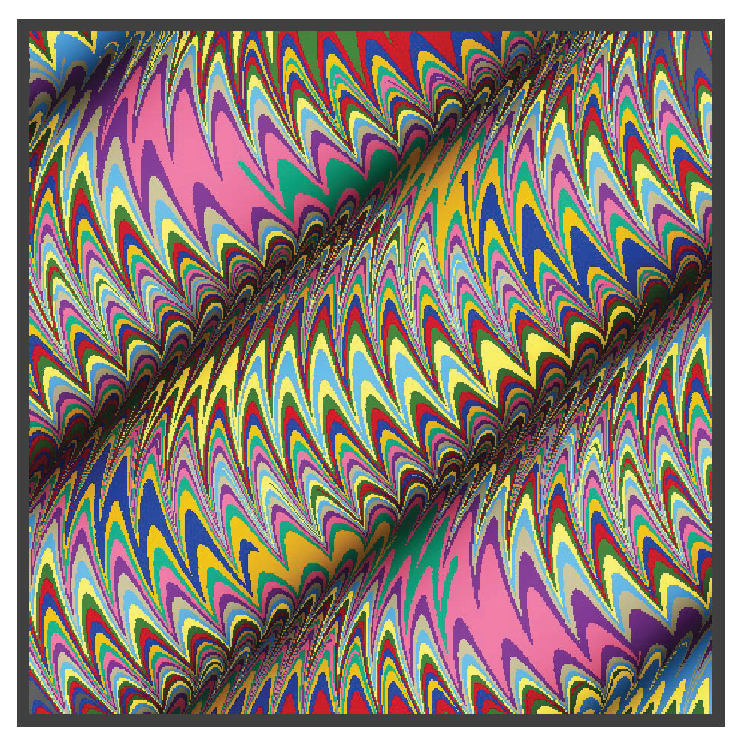
\includegraphics{Rollers.eps}
%\begin{pspicture}(-6,-6)(6,6)
%  \psMarble[
%    background={
%      [64 64 64]
%    },
%    colors={
%      [0.275 0.569 0.796][0.965 0.882 0.302]
%      [0.176 0.353 0.129][0.635 0.008 0.094]
%      [0.078 0.165 0.518][0.824 0.592 0.031]
%      [0.059 0.522 0.392][0.816 0.333 0.475]
%      [0.365 0.153 0.435][0.624 0.588 0.439]
%    },
%    viscosity=1000,
%    oversample=1.5,
%    actions={
%      0 0 48 colors 25 concentric-rings
%      90  [-150 450] 100 750 31 rake
%      -90 [-150 450] 100 750 31 rake
%      180 [ 25 50 0 tines ] 30 200 31 rake
%      0 230 shift
%      -40 400 0 90 90 jiggle
%    },
%    shadings={
%      -40 400 0 90 jiggle-shade
%    }
%  ](-6,-6)(6,6)
%\end{pspicture}
\end{center}
{\small\begin{verbatim}
\begin{pspicture}(-6,-6)(6,6)
  \psMarble[
    background={[64 64 64]},
    colors={
      [0.275 0.569 0.796][0.965 0.882 0.302]
      [0.176 0.353 0.129][0.635 0.008 0.094]
      [0.078 0.165 0.518][0.824 0.592 0.031]
      [0.059 0.522 0.392][0.816 0.333 0.475]
      [0.365 0.153 0.435][0.624 0.588 0.439]
    },
    viscosity=1000,oversample=1.5,
    actions={
      0 0 48 colors 25 concentric-rings
      90  [-150 450] 100 750 31 rake
      -90 [-150 450] 100 750 31 rake
      180 [ 25 50 0 tines ] 30 200 31 rake
      0 230 shift
      -40 400 0 90 90 jiggle
    },
    shadings={
      -40 400 0 90 jiggle-shade
    }
  ](-6,-6)(6,6)
\end{pspicture}
\end{verbatim}}


\newpage


\textbf{Example 13: French Curl}

\begin{center}
\begin{pspicture}(-6,-6)(6,6)
  \psMarble[
    background={
      [ 100 40 40 ]
    },
    colors={
      [ 76 95 63 ]
      [ 53 97 122 ]
      [ 128 78 46 ]
    },
    oversample=1,
    actions={
    0 0 1000 1000 0 [ 222 186 149 ]  85 1.72 10 mul uniform-drops
    0 0 1000 1000 0 colors          250 1.72 16 mul uniform-drops
    0 0 1000 1000 0 [ 222 186 149 ] 100 1.72  7 mul uniform-drops
    0 0 [ 100 ] 40 300 31 stir
    0 0 [ 200 275 ] 20 120 10 stir
    0 0 [ 325 ] 20 90 31 stir
    }
  ](12,12)
\end{pspicture}
\end{center}
{\small\begin{verbatim}
\begin{pspicture}(-6,-6)(6,6)
  \psMarble[
    background={
      [ 100 40 40 ]
    },
    colors={
      [ 76 95 63 ]
      [ 53 97 122 ]
      [ 128 78 46 ]
    },
    oversample=1,
    actions={
    0 0 1000 1000 0 [ 222 186 149 ]  85 1.72 10 mul uniform-drops
    0 0 1000 1000 0 colors          250 1.72 16 mul uniform-drops
    0 0 1000 1000 0 [ 222 186 149 ] 100 1.72  7 mul uniform-drops
    0 0 [ 100 ] 40 300 31 stir
    0 0 [ 200 275 ] 20 120 10 stir
    0 0 [ 325 ] 20 90 31 stir
    }
  ](12,12)
\end{pspicture}
\end{verbatim}}


\newpage


\textbf{Example 14: Spanish Wave}

\begin{center}
\includegraphics{Wave.eps}
%\begin{pspicture}(-6,-6)(6,6)
%  \psMarble[
%    background={
%      [ 125 53 78 ]
%    },
%    colors={
%      [ 81 118 118 ]
%      [ 232 196 89 ]
%    },
%    viscosity=1000,
%    oversample=1,
%    actions={
%      0 0 800 800 0 colors 1 get 120 25 uniform-drops
%      90 [ 10 100 25 tines ] 40 200 31 rake
%      -90 185 shift
%      0 [ 10 100 25 tines ] 40 200 31 rake
%      180 185 shift
%      -90 [10 100 25 tines ] 40 200 31 rake
%      90 185 shift
%      180 [10 100 25 tines ] 40 200 31 rake
%      0 185 shift
%      0 0 1000 1000 0 [ colors 0 get dup 0.9 shade ] 110 50 uniform-drops
%      -51 120 0 -25 -10 jiggle
%      -49 93 37 -30 -12 jiggle
%    },
%    shadings={
%      -51 120 0 -10 jiggle-shade
%      -49 93 37 -12 jiggle-shade
%    },
%    spractions={
%      0 0 1000 1000 0 [ colors 0 get 1.3 shade ] 1000 1.5 uniform-spray
%    }
%  ](12,12)
%\end{pspicture}
\end{center}
{\tiny\begin{verbatim}
\begin{pspicture}(-6,-6)(6,6)
  \psMarble[
    background={
      [ 125 53 78 ]
    },
    colors={
      [ 81 118 118 ]
      [ 232 196 89 ]
    },
    viscosity=1000,
    oversample=1,
    actions={
      0 0 800 800 0 colors 1 get 120 25 uniform-drops
      90 [ 10 100 25 tines ] 40 200 31 rake
      -90 185 shift
      0 [ 10 100 25 tines ] 40 200 31 rake
      180 185 shift
      -90 [10 100 25 tines ] 40 200 31 rake
      90 185 shift
      180 [10 100 25 tines ] 40 200 31 rake
      0 185 shift
      0 0 1000 1000 0 [ colors 0 get dup 0.9 shade ] 110 50 uniform-drops
      -51 120 0 -25 -10 jiggle
      -49 93 37 -30 -12 jiggle
    },
    shadings={
      -51 120 0 -10 jiggle-shade
      -49 93 37 -12 jiggle-shade
    },
    spractions={
      0 0 1000 1000 0 [ colors 0 get 1.3 shade ] 1000 1.5 uniform-spray
    }
  ](12,12)
\end{pspicture}
\end{verbatim}}


\newpage


\textbf{Example 15: Nautilus}

\begin{center}
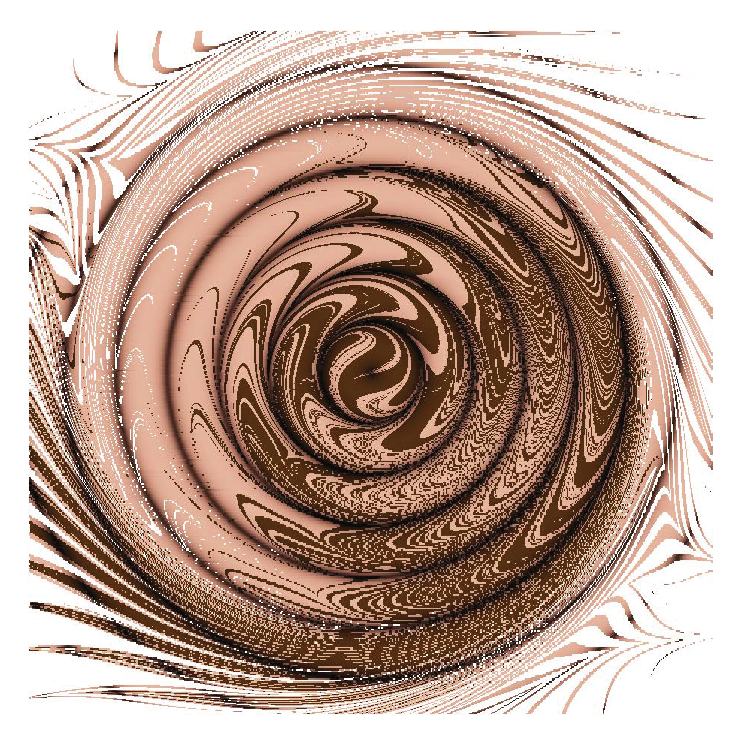
\includegraphics{Nautilus.eps}
%\begin{pspicture}(-6,-6)(6,6)
%  \psMarble[
%    colors={
%      [0.20 0.10 0.02]
%      [0.72 0.49 0.41]
%    },
%    viscosity=1000,
%    oversample=2,
%    actions={
%      0 0 384 colors 1 get drop
%      -192 0 288 colors 0 get drop
%      -192 0 144 colors 1 get drop
%      -192 0 56 colors 0 get drop
%      180 [ -480 80 480 {} for ] 4 150 50 rake
%      0 [ -520 80 520 {} for ] 4 150 50 rake
%      -90 [ -480 80 480 {} for ] 4 150 50 rake
%      90 [ -520 80 520 {} for ] 4 150 50 rake
%      0 0 [ 75 150 225 300 375 ] 4 -120 50 stir
%      0 0 -15 turn
%    },
%    shadings={
%      0 0 -75 0 20 wriggle-shade
%    }
%  ](12,12)
%\end{pspicture}
\end{center}
{\small\begin{verbatim}
\begin{pspicture}(-6,-6)(6,6)
  \psMarble[
    colors={
      [0.20 0.10 0.02]
      [0.72 0.49 0.41]
    },
    viscosity=1000,
    oversample=2,
    actions={
      0 0 384 colors 1 get drop
      -192 0 288 colors 0 get drop
      -192 0 144 colors 1 get drop
      -192 0 56 colors 0 get drop
      180 [ -480 80 480 {} for ] 4 150 50 rake
      0 [ -520 80 520 {} for ] 4 150 50 rake
      -90 [ -480 80 480 {} for ] 4 150 50 rake
      90 [ -520 80 520 {} for ] 4 150 50 rake
      0 0 [ 75 150 225 300 375 ] 4 -120 50 stir
      0 0 -15 turn
    },
    shadings={
      0 0 -75 0 20 wriggle-shade
    }
  ](12,12)
\end{pspicture}
\end{verbatim}}


\newpage


\textbf{Example 16: Moire}

\begin{center}
\begin{pspicture}(-6,-6)(6,6)
  \psMarble[
    background={
      [ 0 0 0 ]
    },
    paper={
      [ 0 0 0 ]
    },
    colors={
      [ 245 245 245 ]
      [ 31 133 241 ]
      [ 248 159 241 ]
    },
    viscosity=1000,
    oversample=1,
    actions={
      0 0 850 850 0 colors 0 get 150 20 uniform-drops
      0 0 950 950 0 colors 1 get 150 20 uniform-drops
      0 0 1050 1050 0 colors 2 get 150 20 uniform-drops
      0 -1000 300 95 1 wriggle
    },
    shadings={
      0 -1000 300 0 90 wriggle-shade
    }
  ](12,12)
\end{pspicture}
\end{center}
{\small\begin{verbatim}
\begin{pspicture}(-6,-6)(6,6)
  \psMarble[
    background={
      [ 0 0 0 ]
    },
    paper={
      [ 0 0 0 ]
    },
    colors={
      [ 245 245 245 ]
      [ 31 133 241 ]
      [ 248 159 241 ]
    },
    viscosity=1000,
    oversample=1,
    actions={
      0 0 850 850 0 colors 0 get 150 20 uniform-drops
      0 0 950 950 0 colors 1 get 150 20 uniform-drops
      0 0 1050 1050 0 colors 2 get 150 20 uniform-drops
      0 -1000 300 95 1 wriggle
    },
    shadings={
      0 -1000 300 0 90 wriggle-shade
    }
  ](12,12)
\end{pspicture}
\end{verbatim}}



\textbf{Example 17: Blendmodes}

In case one want to overlap various marblings one can use the following blendmodes (basic option in PSTricks):

\texttt{/Normal: blendmode=0},
\texttt{/Compatible: blendmode=1},
\texttt{/Screen: blendmode=2},
\texttt{/Multiply: blendmode=3},

\texttt{/HardLight: blendmode=4},
\texttt{/Darken: blendmode=5},
\texttt{/Lighten: blendmode=6},
\texttt{/Difference: blendmode=7},

\texttt{/ColorDodge: blendmode=8},
\texttt{/ColorBurn: blendmode=9},
\texttt{/SoftLight: blendmode=10},
\texttt{/Hue: blendmode=11},

\texttt{/Saturation: blendmode=12},
\texttt{/Luminosity: blendmode=13},
\texttt{/Overlay: blendmode=14},

\texttt{/Exclusion: blendmode=15},
\texttt{/Color: blendmode=16}.

Just set
\begin{verbatim}
\psMarble[blendmode=5,shapealpha=1, ...]
\end{verbatim}

\medskip

\begin{center}
\begin{pspicture}(-4,-4)(4,4)
\pstVerb{%
[ /BM /Darken /ca 1 /CA 1 /SetTransparency pdfmark
}
\psMarble[viscosity=1000,
actions={
0 0 400 400 0 [1 0 0] 10 25 normal-drops
0 0 400 400 0 [0.7 0.5 0] 50 20 normal-drops
0 0 400 400 0 [0 0 0.5] 15 36 normal-drops
}](8,8)
\psMarble[viscosity=1000,bckg=false,
actions={
      -300 92 500
      {
        0 exch 90 [ 12 100 -100 tines ] [ 76 95 63 ] 45 line-drops
      } for
    90 [11 200 0 tines] 40 200 31 rake
    -90 [11 200 0 tines] 40 200 31 rake
    0 0 [-350] 30 30 15 stir
    0 0 [-150] 60 30 15 stir
    }](8,8)
\end{pspicture}
\end{center}
{\small\begin{verbatim}
\begin{pspicture}(-4,-4)(4,4)
\psMarble[blendmode=5,shapealpha=1,viscosity=1000,
actions={
0 0 400 400 0 [1 0 0] 10 25 normal-drops
0 0 400 400 0 [0.7 0.5 0] 50 20 normal-drops
0 0 400 400 0 [0 0 0.5] 15 36 normal-drops
}](8,8)
\psMarble[blendmode=5,shapealpha=1,viscosity=1000,bckg=false,
actions={
      -300 92 500
      {
        0 exch 90 [ 12 100 -100 tines ] [ 76 95 63 ] 45 line-drops
      } for
    90 [11 200 0 tines] 40 200 31 rake
    -90 [11 200 0 tines] 40 200 31 rake
    0 0 [-350] 30 30 15 stir
    0 0 [-150] 60 30 15 stir
    }](8,8)
\end{pspicture}
\end{verbatim}}


\newpage


\textbf{Example 18: Transparency}

In case one want to overlap various marblings one can also use transparency, which is a basic option in PSTricks \texttt{opacity=}. Just set
\begin{verbatim}
\psMarble[opacity=0.45, ...]
\end{verbatim}
The values need to be from 0 to 1.


%The transparency is setup right after \texttt{actions=\{} like: \texttt{0.45 .setopacityalpha} or some other value between 0 and 1.
%
%For Distiller users we set the equivalent: \texttt{[ /ca 0.45 /CA 0.45 /SetTransparency pdfmark}

\medskip

\begin{center}
\begin{pspicture}(-4,-4)(4,4)
\pstVerb{%
[ /ca 0.35 /CA 0.35 /SetTransparency pdfmark
}
\psMarble[viscosity=1000,
actions={
0 0 400 400 0 [1 0 0] 10 25 normal-drops
0 0 400 400 0 [0.7 0.5 0] 50 20 normal-drops
0 0 400 400 0 [0 0 0.5] 15 36 normal-drops
}](8,8)
\psMarble[viscosity=1000,bckg=false,
actions={
      -300 92 500
      {
        0 exch 90 [ 12 100 -100 tines ] [ 76 95 63 ] 45 line-drops
      } for
    90 [11 200 0 tines] 40 200 31 rake
    -90 [11 200 0 tines] 40 200 31 rake
    0 0 [-350] 30 30 15 stir
    0 0 [-150] 60 30 15 stir
    }](8,8)
\pstVerb{%
[ /ca 1 /CA 1 /SetTransparency pdfmark
}
\end{pspicture}
\end{center}
{\small\begin{verbatim}
\begin{pspicture}(-4,-4)(4,4)
\psMarble[opacity=0.35,viscosity=1000,
actions={
0 0 400 400 0 [1 0 0] 10 25 normal-drops
0 0 400 400 0 [0.7 0.5 0] 50 20 normal-drops
0 0 400 400 0 [0 0 0.5] 15 36 normal-drops
}](8,8)
\psMarble[opacity=0.35,viscosity=1000,bckg=false,
actions={
      -300 92 500
      {
        0 exch 90 [ 12 100 -100 tines ] [ 76 95 63 ] 45 line-drops
      } for
    90 [11 200 0 tines] 40 200 31 rake
    -90 [11 200 0 tines] 40 200 31 rake
    0 0 [-350] 30 30 15 stir
    0 0 [-150] 60 30 15 stir
    }](8,8)
\end{pspicture}
\end{verbatim}}


\newpage


\section{Acknowledgments}

Many thanks to D. P. Story who coded some additions to the \texttt{pst-marble.pro} file so it might be used for Adobe Distiller users.

The file size for the documentation could so be reduced tremendously.

\bigskip

Also many thanks to A. Grahn who sent a patch to use transparency and blendmode effects with the usual PSTricks options.

%\newpage
%
%
%\section{List of all optional arguments for \texttt{pst-marble}}
%
%\xkvview{family=pst-marble,columns={key,type,default}}
%
%\clearpage
%
%\nocite{*}
%\bgroup
%\RaggedRight
%\printbibliography
%\egroup
%
%\printindex
\end{document}
